\documentclass[12pt,letterpaper]{article}

% ── Fonts & Layout ─────────────────────────────────────────────
\usepackage[margin=0.85in]{geometry}
\usepackage[T1]{fontenc}
\usepackage[utf8]{inputenc}
\usepackage{helvet}
\renewcommand{\familydefault}{\sfdefault}
\usepackage{microtype}
\usepackage{setspace}
\setstretch{1.45}

% ── Packages ──────────────────────────────────────────────────
\usepackage{enumitem}
\usepackage{tabularx}
\usepackage{booktabs}
\usepackage{graphicx}
\usepackage{float}
\usepackage{amsmath}
\usepackage{xcolor}
\usepackage{subcaption}
\usepackage{caption}
\usepackage[hidelinks]{hyperref}

\graphicspath{{figures/}}
\captionsetup{font=small,labelfont=bf,skip=6pt}

\setlist[itemize]{leftmargin=1.5em,noitemsep,topsep=3pt}
\setlist[enumerate]{leftmargin=1.5em,noitemsep,topsep=3pt}

% ── Section formatting ───────────────────────────────────────
\usepackage{titlesec}
\titlespacing*{\section}{0pt}{10pt}{4pt}
\titlespacing*{\subsection}{0pt}{8pt}{3pt}

\begin{document}

% ═══ Compact Title Block (not a full page) ════════════════════
\begin{center}
\vspace*{-0.3cm}
{\Large\bfseries The Effect of Feedback Modality on Speed--Accuracy\\[2pt]Tradeoff in a Visual Target-Selection Task}\\[10pt]
{\normalsize MIE\,286 -- Probability \& Statistics \hfill Winter 2026 \hfill Team 51}\\[4pt]
{\normalsize Markiyan Konyk \quad Jessica Yi \quad Memo Ozdincer}\\[3pt]
{\small University of Toronto \hfill April 7, 2026}
\end{center}
\vspace{0.3cm}
\noindent\rule{\textwidth}{0.4pt}
\vspace{0.3cm}


% ═══ 1. INTRODUCTION ══════════════════════════════════════════
\section{Introduction}

We built a browser-based target-clicking game and asked 72 university students to play it under two different feedback conditions: one where the screen border flashes a color after each click (visual), and one where a tone plays instead (auditory). The question: does the type of feedback change how people balance speed and accuracy?

Figure~\ref{fig:interface} shows the game. A blue target appears at a random position on an 800$\times$500\,px canvas; the participant clicks it as fast and accurately as they can. In the visual condition, the border glows gold (fast hit), green (slow hit), or red (miss). In the auditory condition, a high, medium, or low tone plays instead. Both convey the same three levels of information.

\begin{figure}[H]
\centering
\begin{subfigure}[t]{0.48\textwidth}
  \centering
  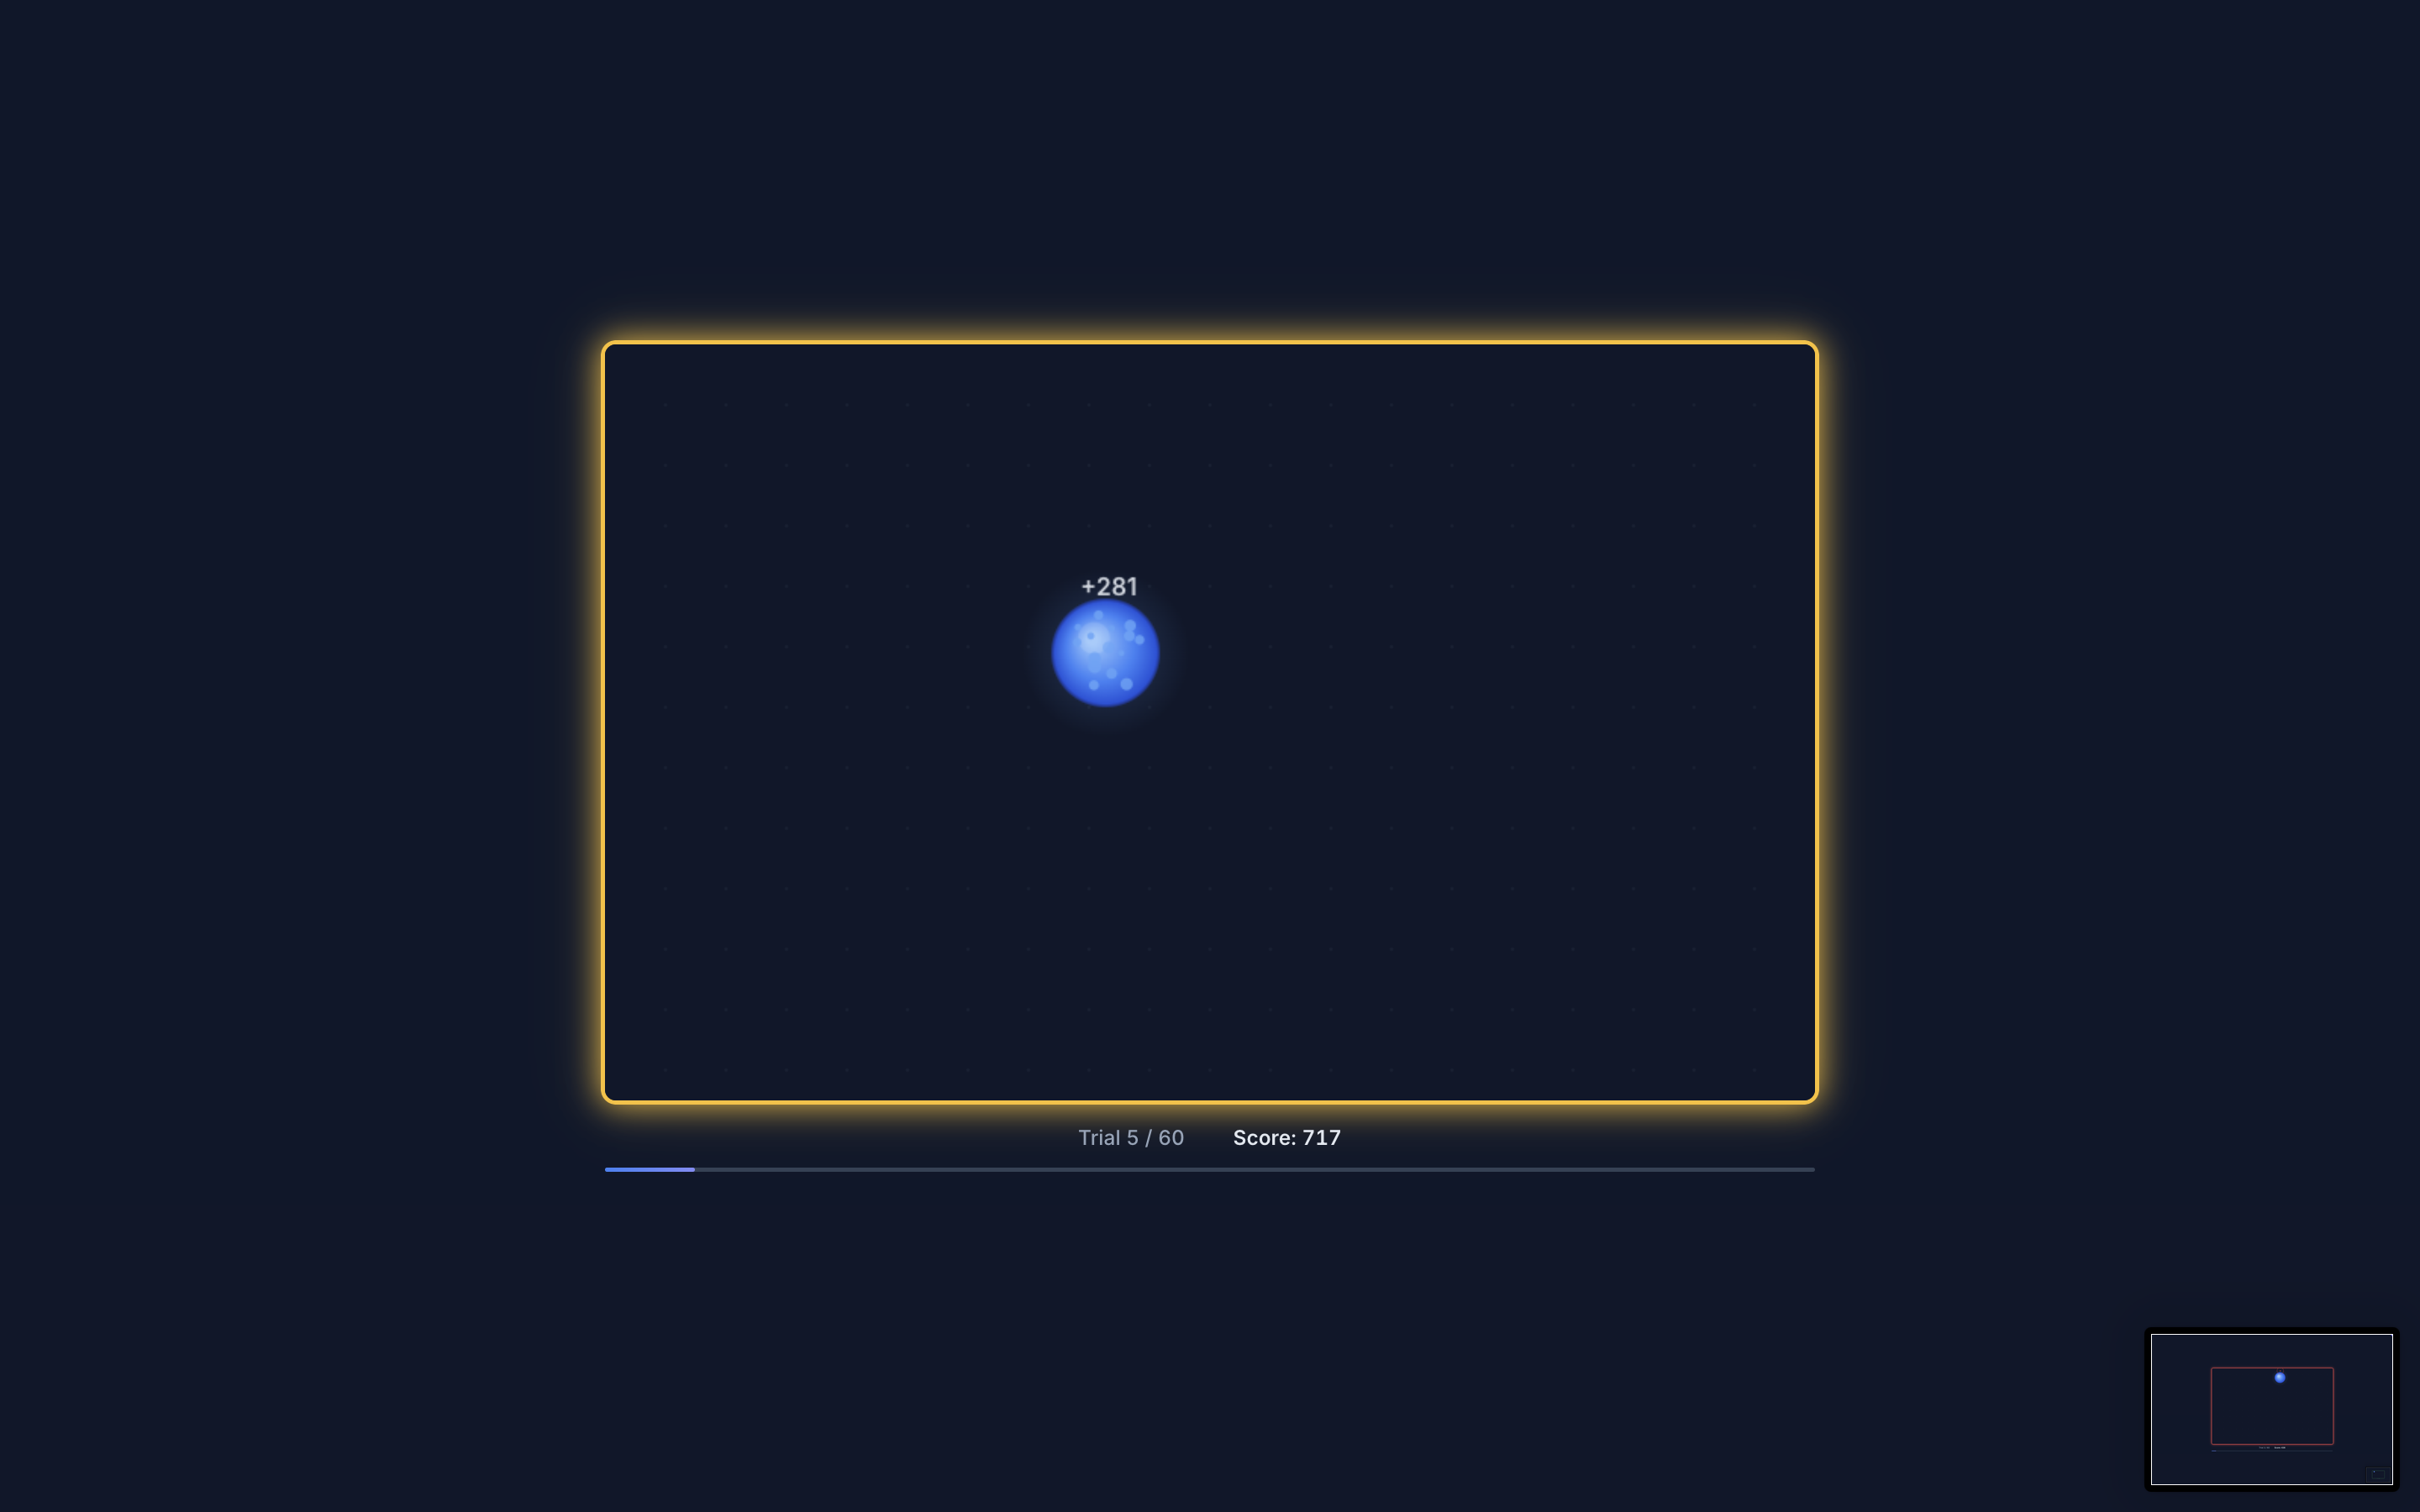
\includegraphics[width=\textwidth]{hit_gold_feedback_visual.png}
  \caption{Visual: gold glow = fast hit ($<$600\,ms)}
\end{subfigure}
\hfill
\begin{subfigure}[t]{0.48\textwidth}
  \centering
  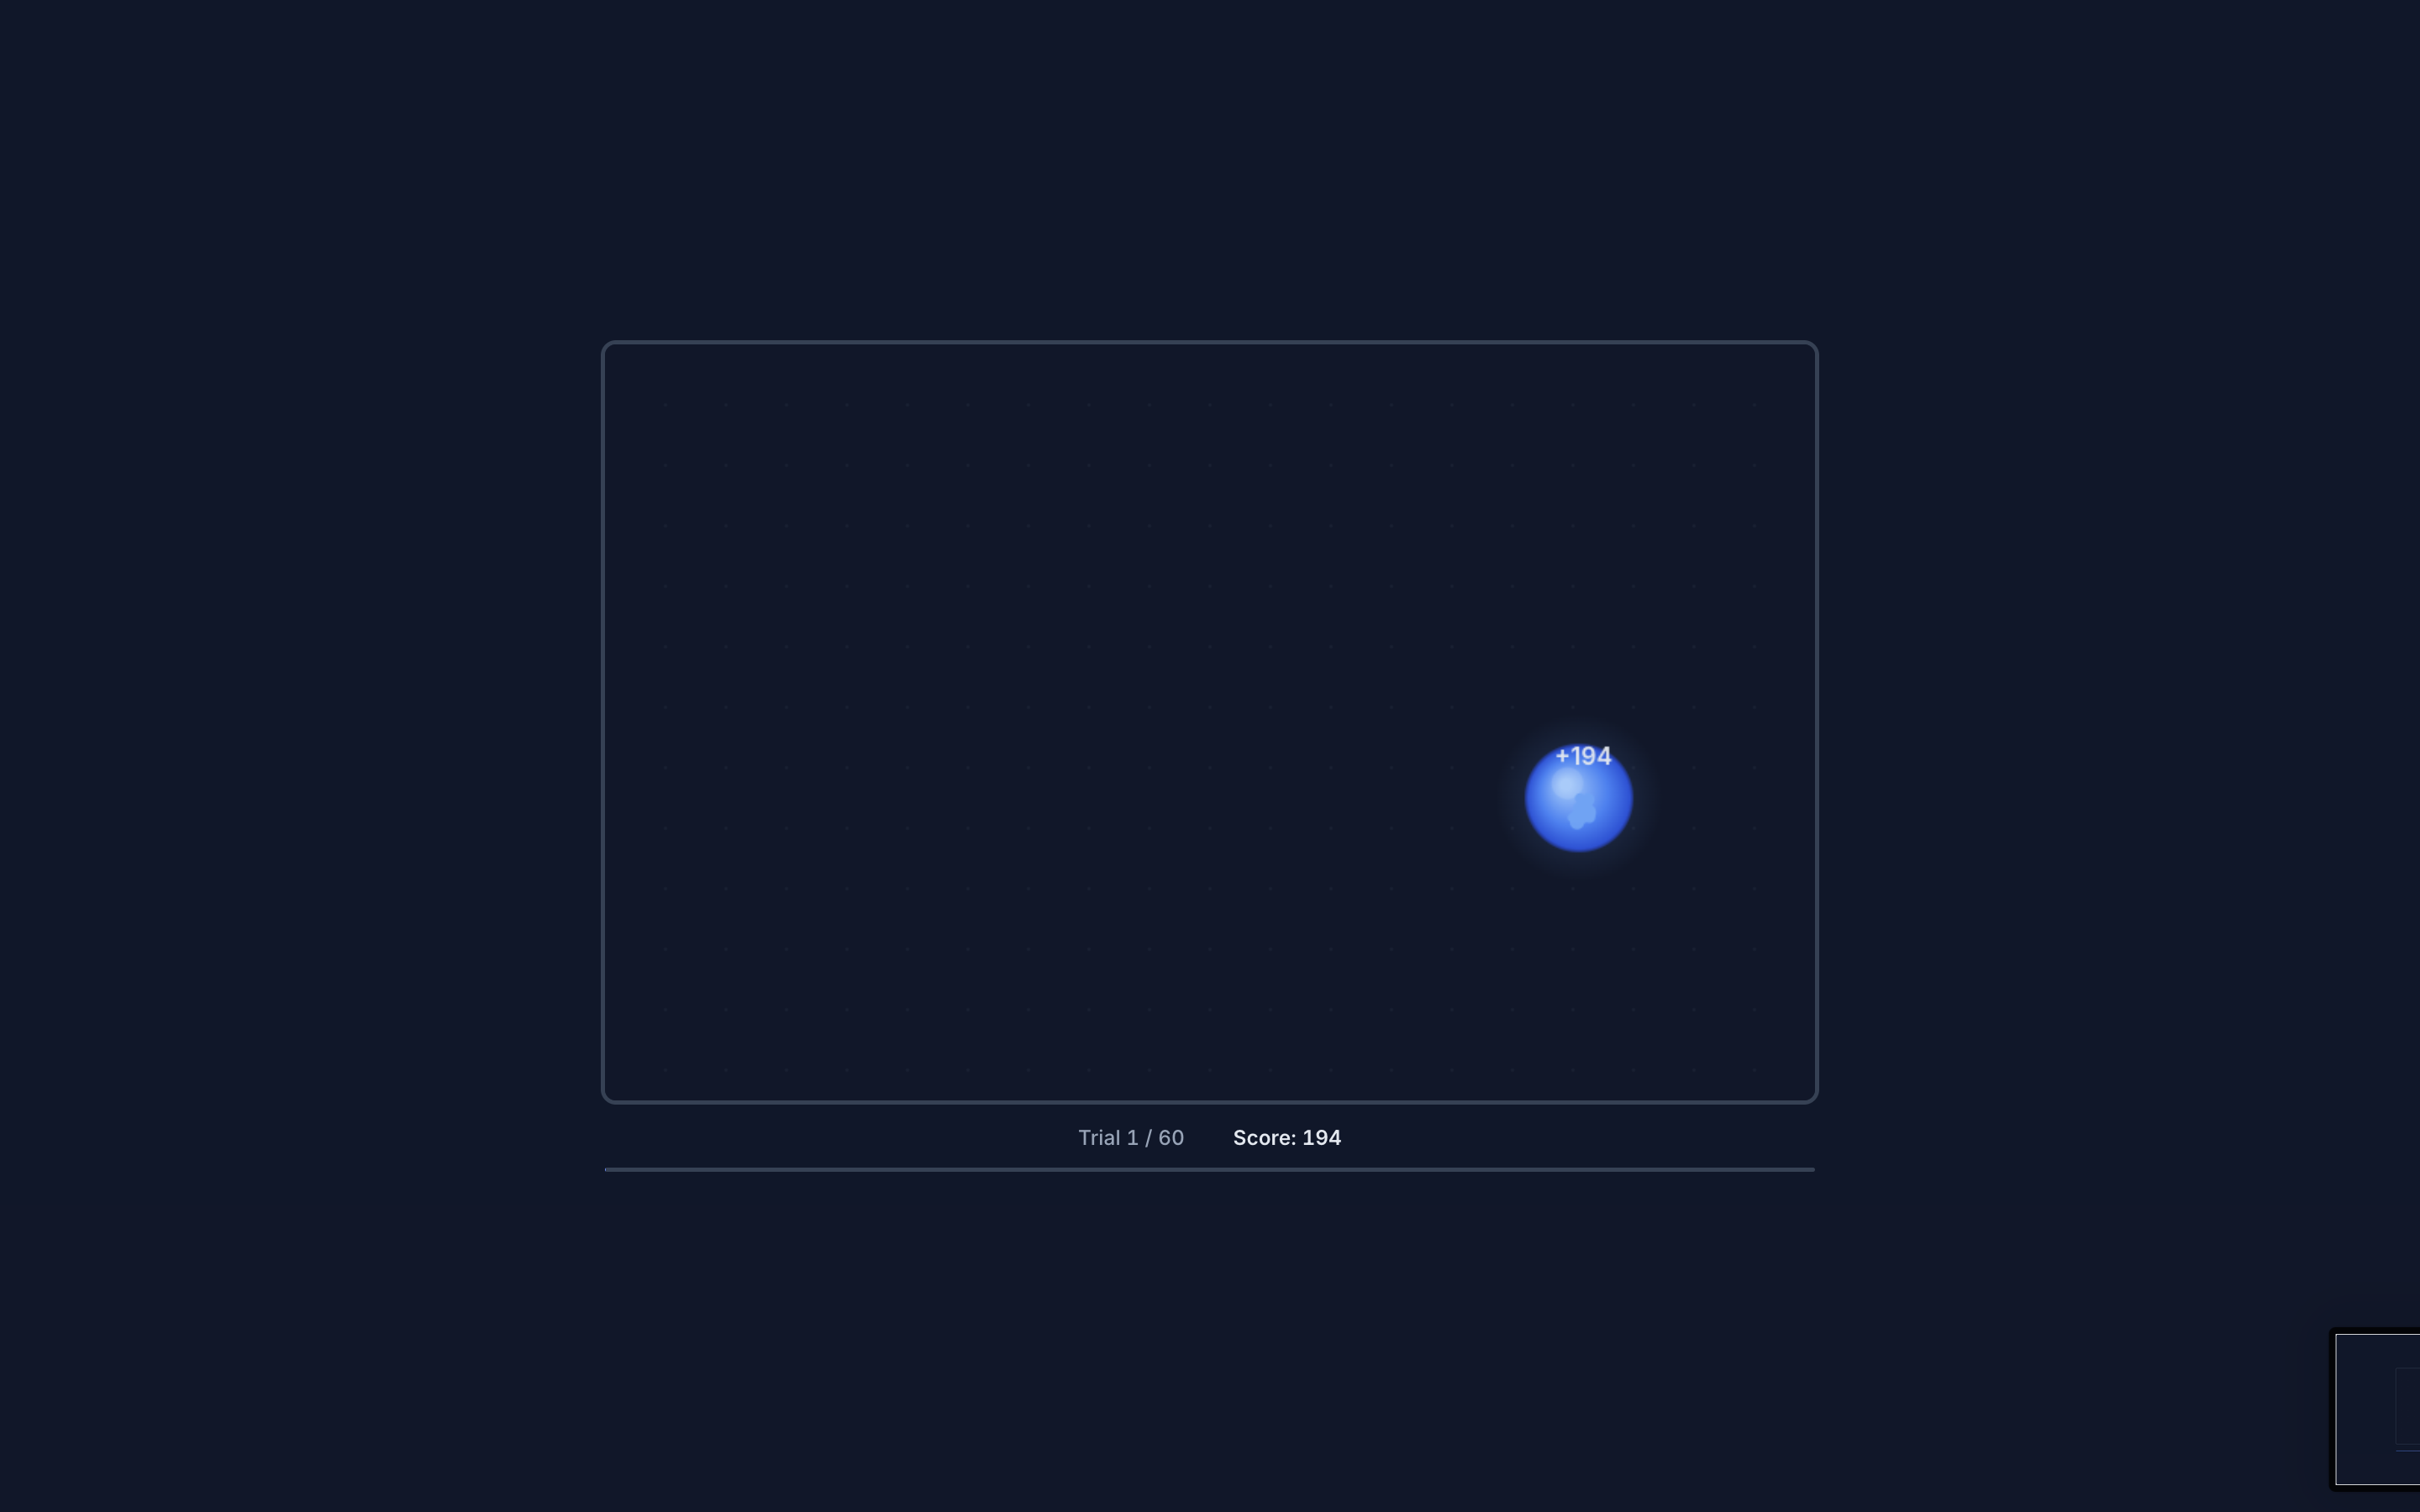
\includegraphics[width=\textwidth]{hit_on_audio_shows_no_visual_confimation.png}
  \caption{Auditory: no visual change, tone plays}
\end{subfigure}
\caption{The experiment interface in both conditions. The only difference is the feedback channel.}
\label{fig:interface}
\end{figure}

Wickens' Multiple Resource Theory~[1,\,2] predicts that a visual task paired with visual feedback should overload one attentional channel, making auditory feedback less disruptive. Cognitive Load Theory~[3] agrees: distributing information across modalities should reduce burden. We expected auditory feedback to produce faster, more efficient responses.

What we found was the opposite. Visual feedback made people \emph{faster}, not slower. The gold/green distinction created a visible speed target that participants actively chased---they were frustrated when they got green instead of gold. This motivational effect overrode the predicted interference. We tested three hypotheses:

\begin{enumerate}
  \item \textbf{H\textsubscript{1}:} Reaction time will differ between visual and auditory feedback.
  \item \textbf{H\textsubscript{2}:} The faster condition will have greater radial error (speed--accuracy tradeoff).
  \item \textbf{H\textsubscript{3}:} The speed--accuracy tradeoff \emph{structure} (slope of RT vs.\ error) will differ between conditions.
\end{enumerate}


% ═══ 2. BACKGROUND ════════════════════════════════════════════
\section{Background}

The speed--accuracy tradeoff (SAT) is a fundamental constraint: faster responses are generally less accurate. Heitz~[6] emphasizes that the SAT is not a single number but a \emph{function} whose shape can change across conditions. Fitts' Law~[4,\,5] characterizes motor pointing performance, but our task holds target size constant and randomizes position, so differences should reflect cognitive processing of feedback rather than pure motor constraints.

Prior work supports modality effects. Akamatsu et al.~[7] found auditory feedback reduced movement time in pointing tasks. Sigrist et al.~[8] reviewed evidence that auditory feedback supports motor learning through cross-modal facilitation. However, these studies examined mean performance---whether modality changes the SAT \emph{slope} remains open.


% ═══ 3. METHODS ═══════════════════════════════════════════════
\section{Methods}

\subsection{Participants}

72 individuals (ages 18--24, university students) participated via convenience sampling. Table~\ref{tab:sample} summarizes the sample.

\begin{table}[H]
\centering
\caption{Participant demographics and covariates.}
\label{tab:sample}
\begin{tabular}{llr}
\toprule
\textbf{Covariate} & \textbf{Level} & \textbf{$N$} \\
\midrule
\multirow{3}{*}{Input Device} & Mouse & 27 \\
 & Trackpad & 31 \\
 & Other & 14 \\[4pt]
\multirow{4}{*}{Gaming Frequency} & Never & 15 \\
 & Rarely & 23 \\
 & Weekly & 22 \\
 & Daily & 12 \\[4pt]
\multirow{2}{*}{Condition Order} & Visual $\to$ Auditory & 32 \\
 & Auditory $\to$ Visual & 40 \\
\bottomrule
\end{tabular}
\end{table}

\subsection{Apparatus and Task}

The experiment was a browser-based application hosted on GitHub Pages. Targets (radius = 35\,px) appeared at random canvas positions; participants clicked them as quickly and accurately as possible. Timing used the browser's \texttt{performance.now()} API (sub-millisecond precision). A 400\,ms inter-trial interval separated targets. Figure~\ref{fig:feedback_states} shows the three visual feedback states.

\begin{figure}[H]
\centering
\begin{subfigure}[t]{0.31\textwidth}
  \centering
  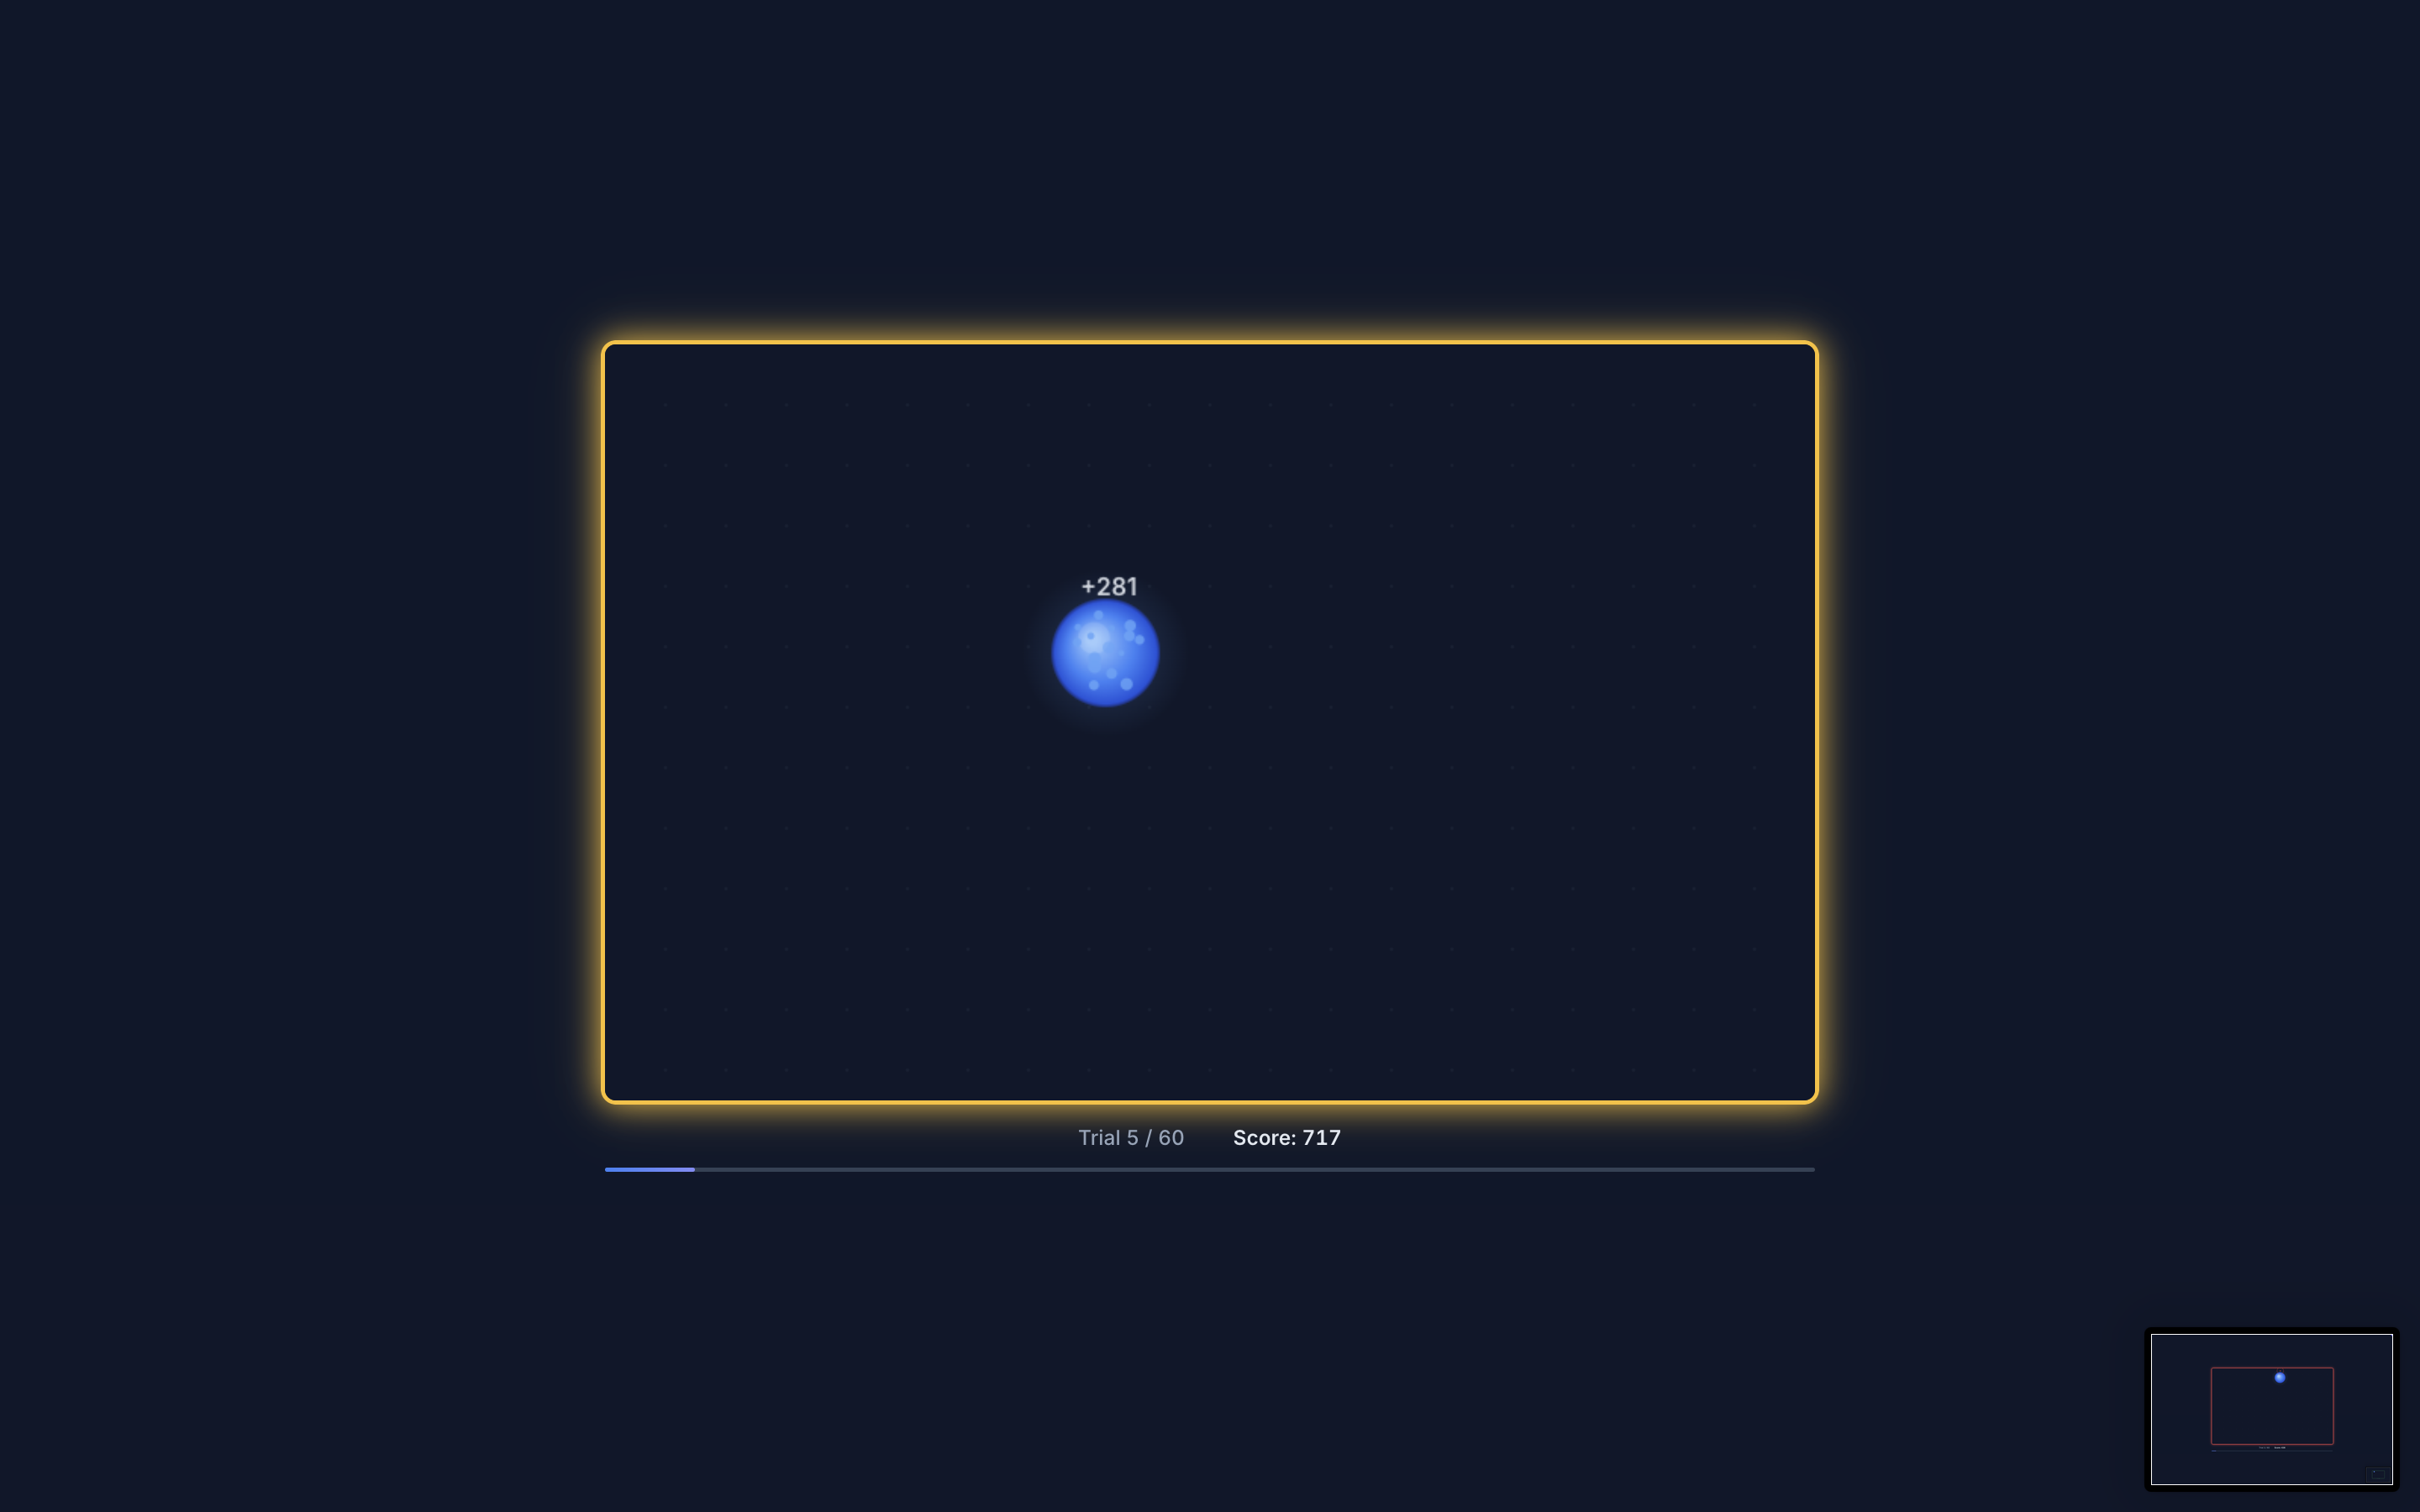
\includegraphics[width=\textwidth]{hit_gold_feedback_visual.png}
  \caption{Gold (fast hit)}
\end{subfigure}
\hfill
\begin{subfigure}[t]{0.31\textwidth}
  \centering
  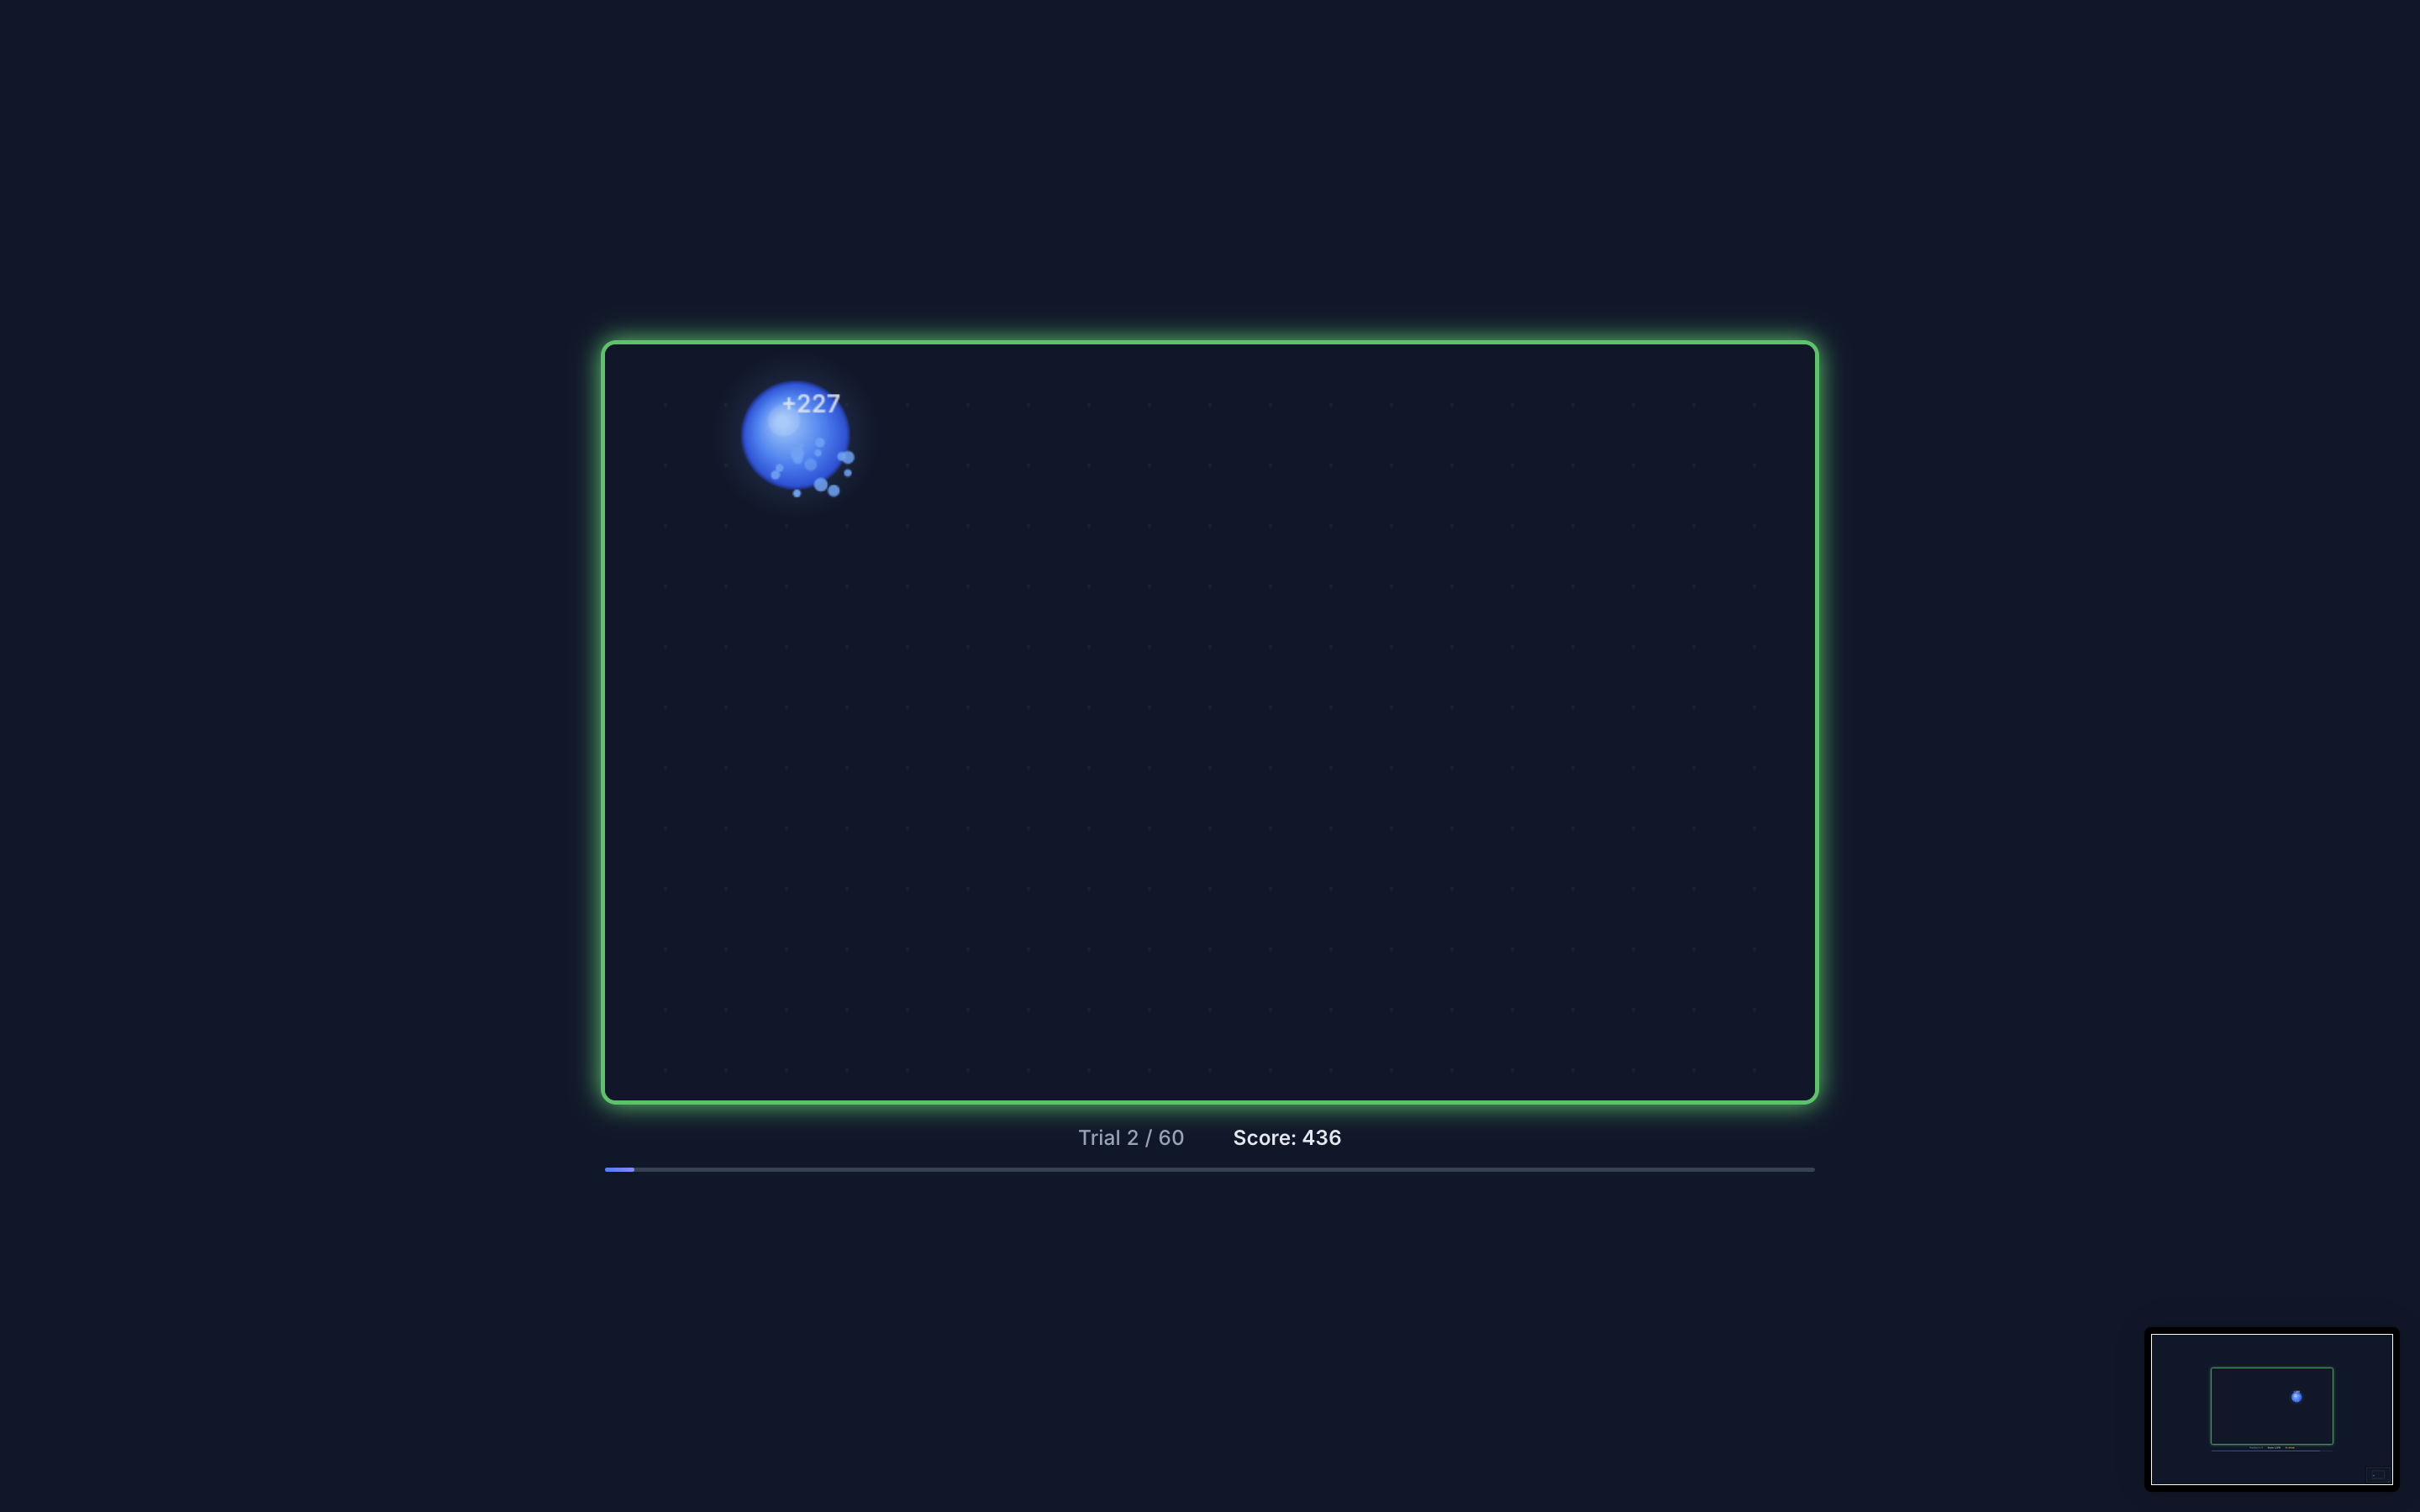
\includegraphics[width=\textwidth]{green_feedback_visual.png}
  \caption{Green (slow hit)}
\end{subfigure}
\hfill
\begin{subfigure}[t]{0.31\textwidth}
  \centering
  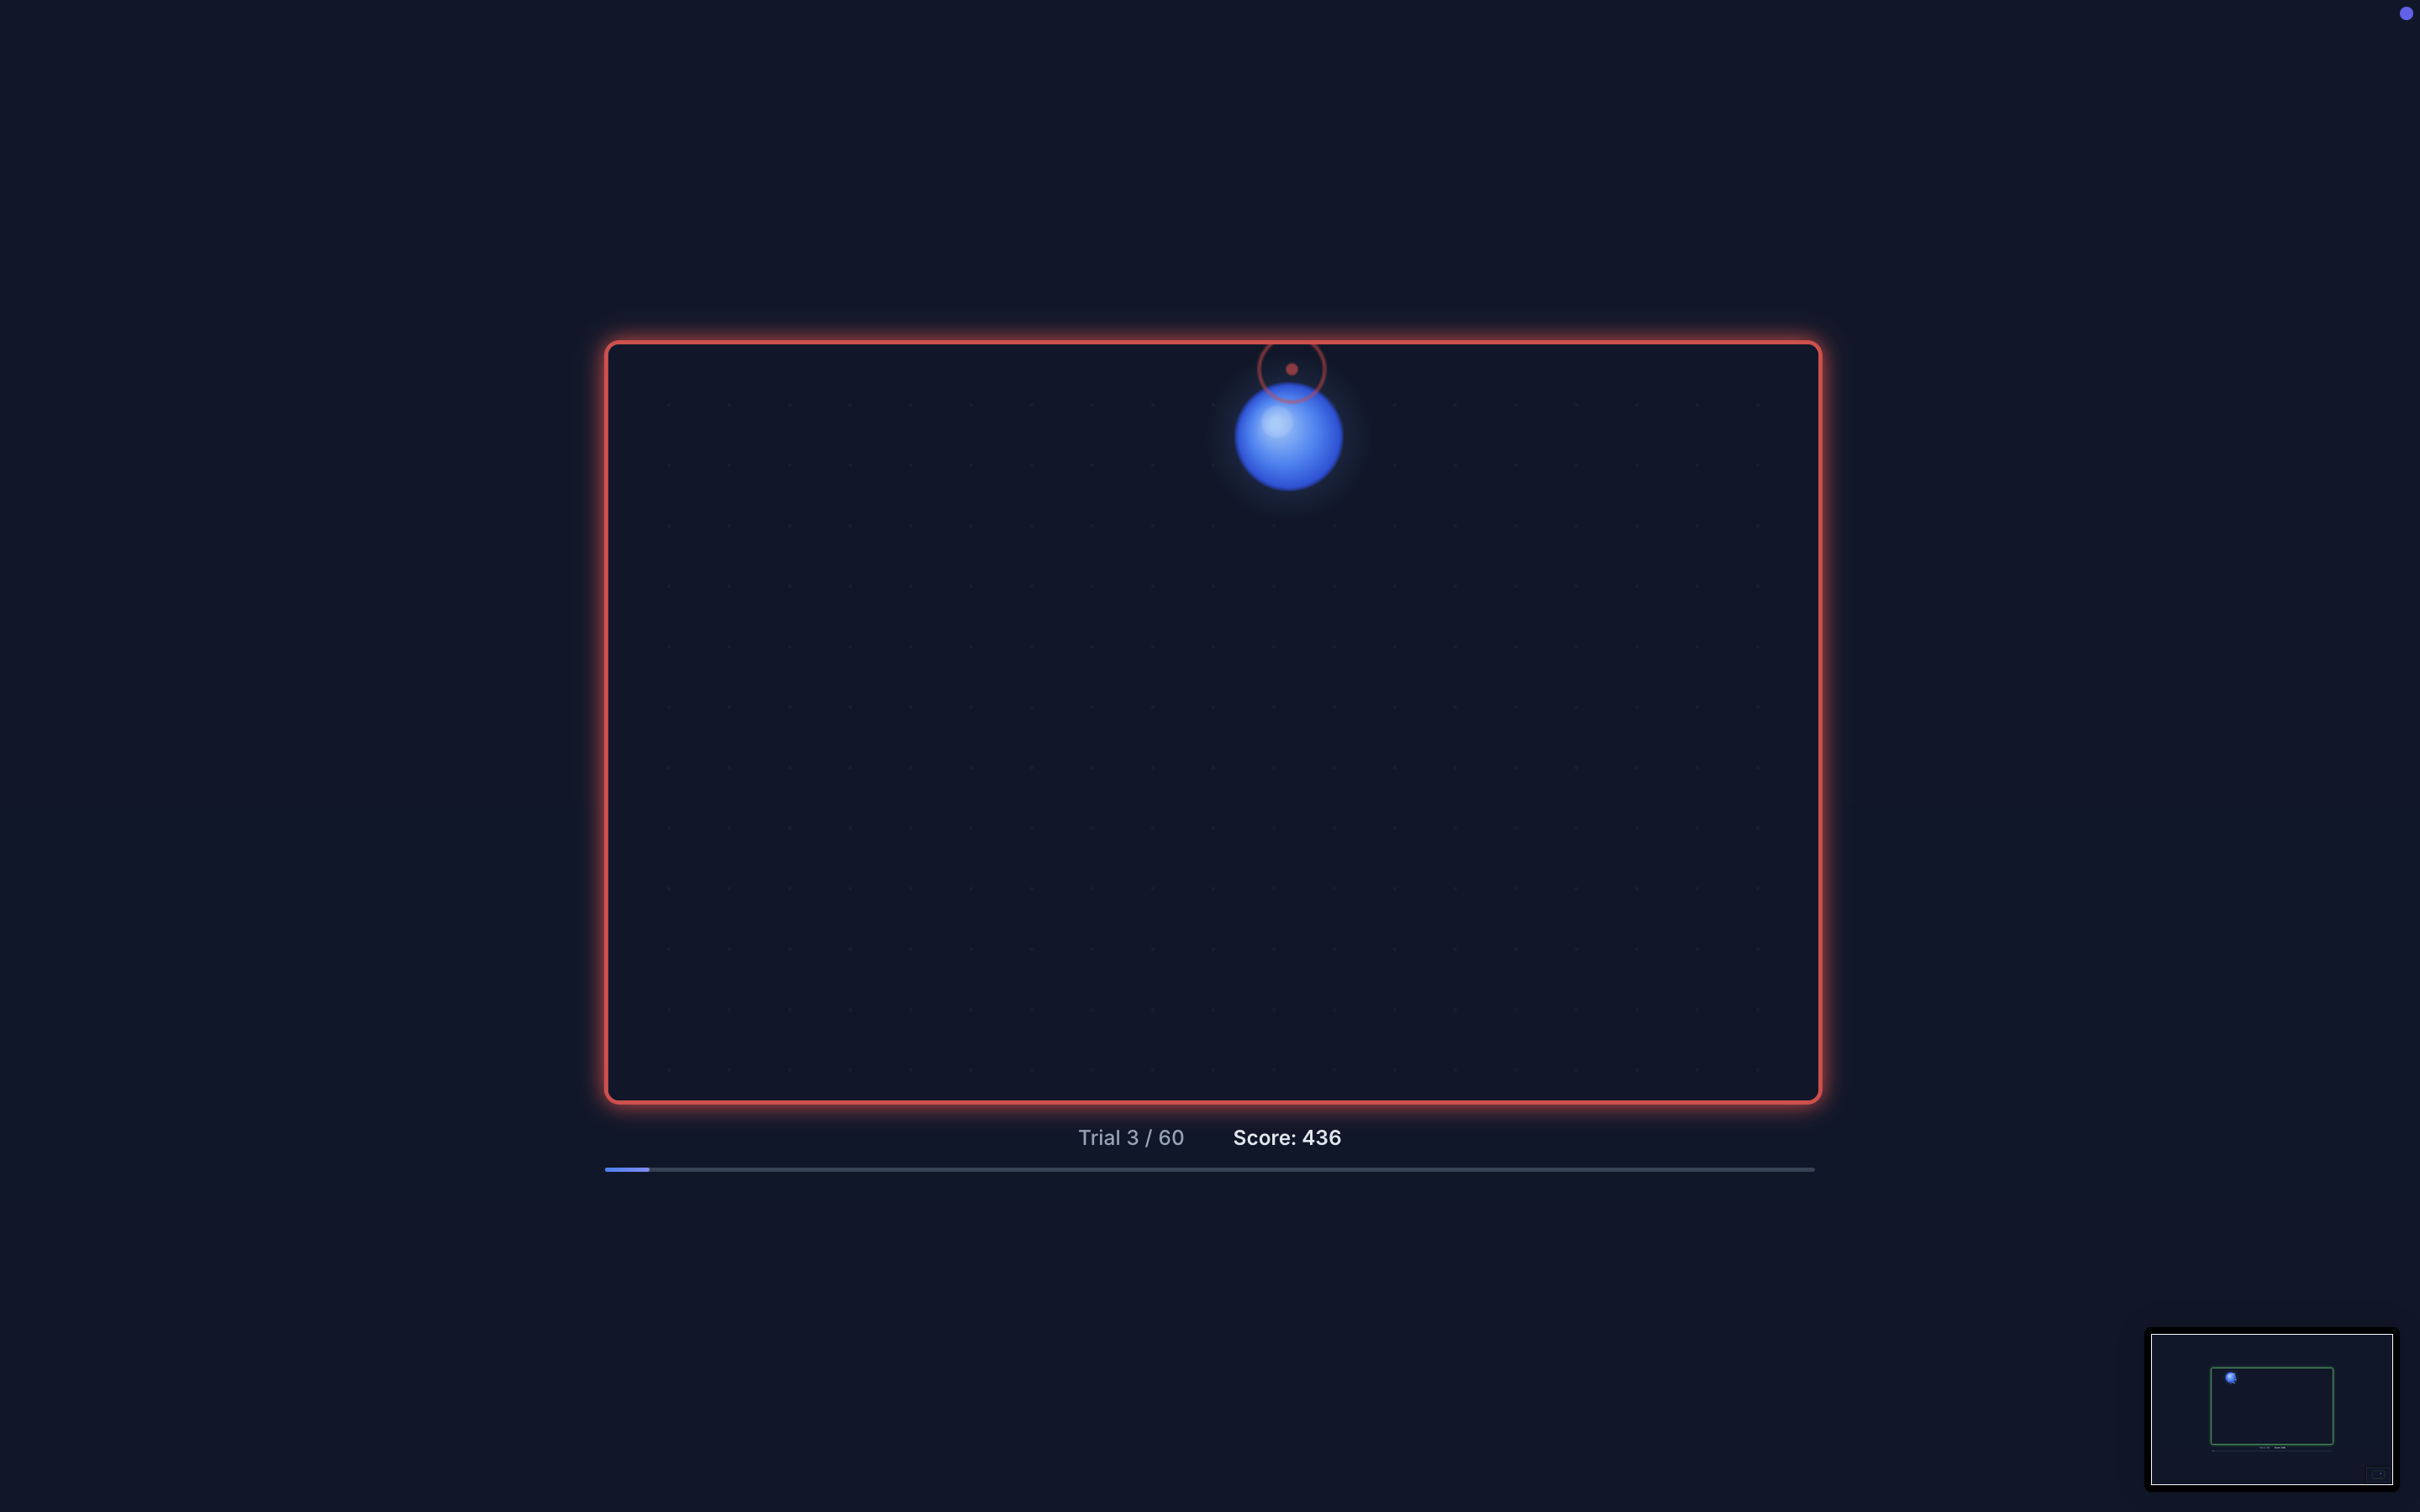
\includegraphics[width=\textwidth]{miss_feedback_visual.png}
  \caption{Red + shake (miss)}
\end{subfigure}
\caption{The three visual feedback states. Gold vs.\ green created a salient speed incentive---participants were observed chasing gold.}
\label{fig:feedback_states}
\end{figure}

\subsection{Independent Variable}

Feedback type was within-subject with two levels:

\textbf{Visual.} Border glow---gold ($<$600\,ms), green ($\geq$600\,ms), or red + shake (miss). 150\,ms duration.

\textbf{Auditory.} Pure tones---880\,Hz (fast hit), 440\,Hz (slow hit), 180\,Hz (miss). 200\,ms duration.

Both conditions conveyed identical three-level information. The on-screen HUD (trial counter, score, streak) was identical in both conditions. This addresses the proposal feedback, which noted an information asymmetry in the original design.

\subsection{Dependent Variables}

\textbf{DV\textsubscript{1}: Reaction time} (ms)---target onset to click.

\textbf{DV\textsubscript{2}: Radial error} (px)---Euclidean distance from click to target center. Hit = error $\leq$ 35\,px.

\subsection{Procedure}

\vspace{4pt}
\noindent
\fbox{\parbox{0.95\textwidth}{\small
Consent $\;\to\;$ Instructions $\;\to\;$ 5 practice trials $\;\to\;$ \textbf{Block 1} (30 or 60 trials) $\;\to\;$ Break $\;\to\;$ \textbf{Block 2} $\;\to\;$ End screen
}}
\vspace{4pt}

Condition order was randomized per participant. Target positions were randomized. A gamification system (scoring, particle effects, and a leaderboard) was introduced mid-collection to boost engagement and recruitment.

\subsection{Potential Biases}

Convenience sampling limits generalizability. Device variability introduced noise (mouse users were 178\,ms faster than trackpad users). Trial counts varied (30 vs.\ 60 per block); per-participant means normalize this. Audio environment was uncontrolled. The leaderboard introduced mid-collection increased speed by 96\,ms ($p < .001$) but did not affect accuracy. Four participants completed the experiment twice; each attempt was treated as a separate observation.


% ═══ 4. ANALYSIS ══════════════════════════════════════════════
\section{Analysis}

\subsection{Data Cleaning}

Trials with RT $< 150$\,ms (anticipatory) or $> 8{,}000$\,ms (inattention) were excluded---77 of 6{,}840 trials (1.13\%). The remaining 6{,}763 trials were aggregated to per-participant means for each condition, yielding 72 paired observations.

\subsection{Assumption Checks}

Normality of within-subject differences was assessed with the Shapiro--Wilk test (Week 10: goodness of fit). RT differences were normal ($W = 0.980$, $p = .304$), so a paired $t$-test was appropriate for H\textsubscript{1}. Error differences were non-normal ($W = 0.420$, $p < .001$) due to heavy tails, so a Wilcoxon signed-rank test was used for H\textsubscript{2}. QQ plots are in Appendix~A.

\subsection{Hypothesis Tests}

\textbf{H\textsubscript{1} (Speed).} Our original prediction, based on MRT, was that auditory feedback would be faster. The data showed the opposite. We used a \emph{two-tailed} paired $t$-test because our directional prediction was reversed:
\vspace{-4pt}
\begin{align*}
  H_0 &: \mu_{\text{vis}} = \mu_{\text{aud}} &\quad H_1 &: \mu_{\text{vis}} \neq \mu_{\text{aud}}
\end{align*}

\textbf{H\textsubscript{2} (Accuracy).} One-tailed Wilcoxon signed-rank test (normality violated):
\vspace{-4pt}
\begin{align*}
  H_0 &: \text{median}(d_{\text{error}}) \leq 0 &\quad H_1 &: \text{median}(d_{\text{error}}) > 0
\end{align*}
where $d = \bar{e}_{\text{vis}} - \bar{e}_{\text{aud}}$ per participant.

\textbf{H\textsubscript{3} (SAT structure).} Multiple linear regression with interaction (Week 12--13):
\[
  \text{error} = \beta_0 + \beta_1 \!\cdot\! \text{RT} + \beta_2 \!\cdot\! \text{condition} + \beta_3 \!\cdot\! (\text{RT} \times \text{condition}) + \varepsilon
\]
A significant $\beta_3$ indicates different SAT slopes. Supplemented with Pearson correlations (Week 2--3) and simple linear regression per condition (Week 11).

All tests used $\alpha = 0.05$. Cohen's $d$ reported for paired comparisons.


% ═══ 5. RESULTS ═══════════════════════════════════════════════
\section{Results}

\subsection{Descriptive Statistics}

Table~\ref{tab:dvs} summarizes the two dependent variables. Visual feedback was associated with faster responses and slightly greater error, consistent with the SAT.

\begin{table}[H]
\centering
\caption{Performance by feedback condition ($N = 72$). Values are means of per-participant means $\pm$ SD.}
\label{tab:dvs}
\begin{tabular}{lccc}
\toprule
& \textbf{Visual} & \textbf{Auditory} & \textbf{Difference} \\
\midrule
Reaction Time (ms) & $683 \pm 133$ & $693 \pm 140$ & $-9.7$ \\
Radial Error (px) & $17.9 \pm 30.5$ & $18.5 \pm 39.6$ & $-0.5$ \\
Hit Rate (\%) & 94.4 & 94.8 & $-0.4$ \\
RT Std Dev (ms) & $132.9$ & $140.2$ & $-7.3$ \\
\bottomrule
\end{tabular}
\end{table}

\subsection{Reaction Time}

Figure~\ref{fig:spaghetti} shows individual participant trajectories. While the grand mean difference is only 9.7\,ms, individual variation is large---some participants were over 100\,ms faster under visual, others 100\,ms slower. This between-participant variability ($SD = 56.5$\,ms) is why H\textsubscript{1} did not reach significance.

\begin{figure}[H]
\centering
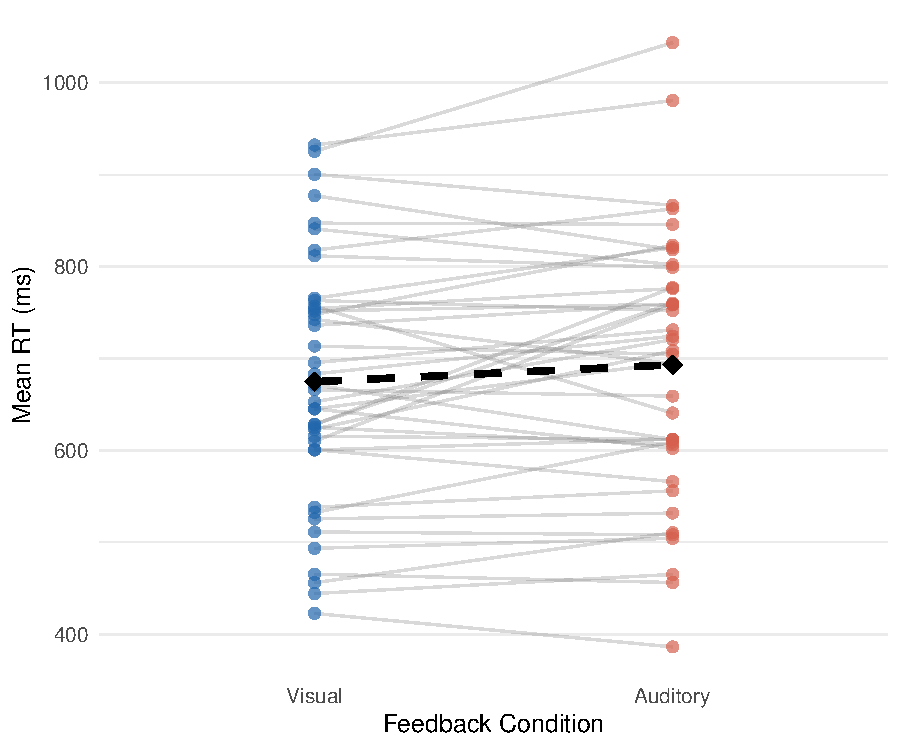
\includegraphics[width=0.7\textwidth]{rt_spaghetti.pdf}
\caption{Paired RT comparison. Each grey line = one participant. Diamond = grand mean. Slopes vary widely.}
\label{fig:spaghetti}
\end{figure}

\textbf{H\textsubscript{1} result.} Paired $t$-test: $t(71) = -1.45$, $p = .151$, 95\% CI $[-23.0,\ 3.6]$\,ms, $d = -0.17$. We fail to reject $H_0$. The 9.7\,ms difference was not statistically reliable.

Figure~\ref{fig:density} overlays trial-level RT distributions. The visual distribution is tighter and more peaked around 500--600\,ms---the gold threshold range---suggesting participants targeted this boundary.

\begin{figure}[H]
\centering
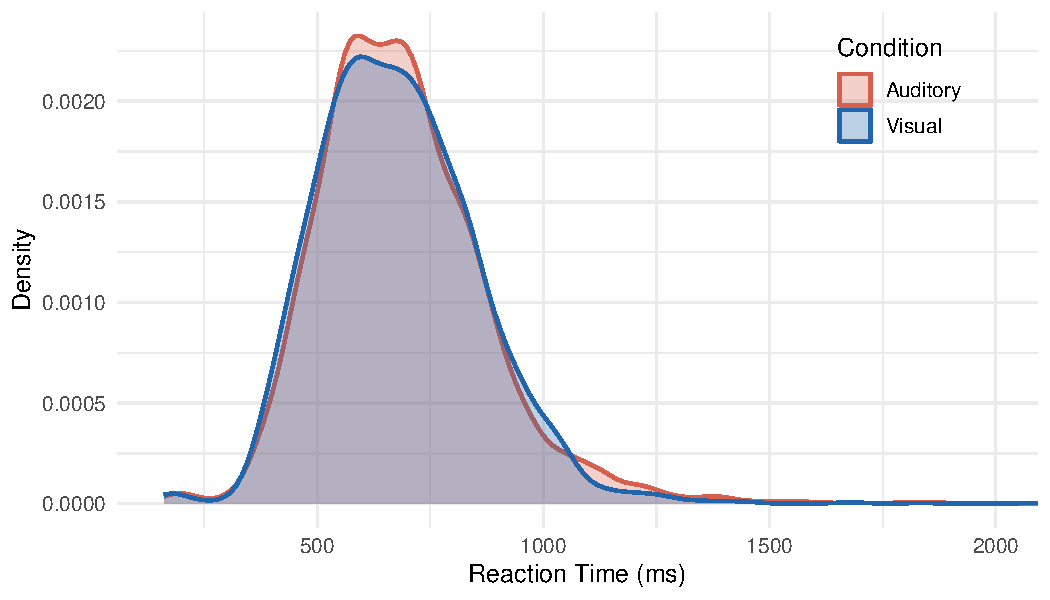
\includegraphics[width=0.75\textwidth]{rt_density.pdf}
\caption{RT distributions by condition. Visual is tighter with a sharper peak near the 600\,ms gold/green threshold.}
\label{fig:density}
\end{figure}

\subsection{Radial Error}

\textbf{H\textsubscript{2} result.} Wilcoxon signed-rank: $V = 1475$, $p = .184$ (one-tailed), $d = -0.05$. Not significant. Accuracy was near ceiling ($\sim$95\% hit rate), limiting the range of detectable error differences.

\subsection{Speed--Accuracy Tradeoff Structure}

This is the central finding. Figure~\ref{fig:sat} shows the SAT scatter---the relationship between RT and radial error at the trial level, with regression lines per condition.

\begin{figure}[H]
\centering
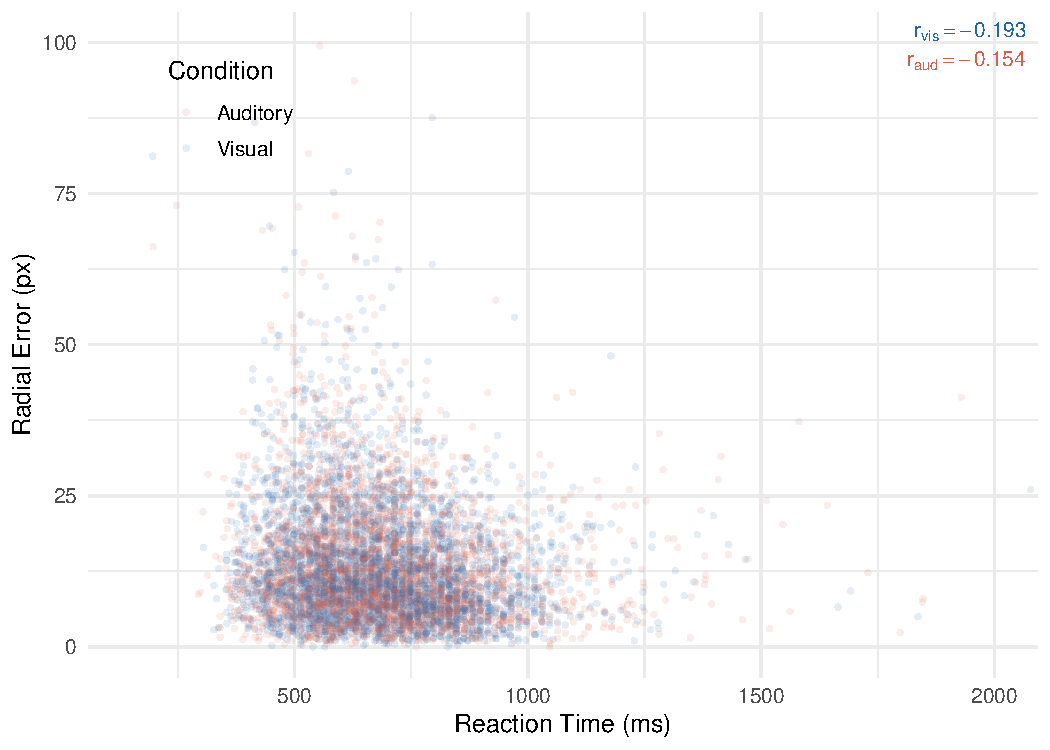
\includegraphics[width=0.85\textwidth]{sat_scatter.pdf}
\caption{Speed--accuracy tradeoff by condition. Each point = one trial. The visual regression line is steeper, meaning faster visual responses incur a larger accuracy penalty. Interaction $p = .023$. Axes capped at 2000\,ms and 100\,px.}
\label{fig:sat}
\end{figure}

\textbf{H\textsubscript{3} result.} The multiple regression interaction was significant: $\beta_3 = -0.0085$, $t(6759) = -2.28$, $p = .023$. The SAT slope under visual feedback ($b = -0.031$, $R^2 = .037$) was 38\% steeper than under auditory ($b = -0.022$, $R^2 = .024$). Pearson correlations: $r_{\text{vis}} = -.193$ ($p < .001$), $r_{\text{aud}} = -.154$ ($p < .001$).

This means visual feedback \emph{amplifies} the tradeoff: each millisecond of speed gained under visual costs more accuracy than under auditory.

\subsection{Covariates}

\begin{table}[H]
\centering
\caption{Performance by input device and gaming frequency.}
\label{tab:covariates}
\begin{tabular}{lccc}
\toprule
& $N$ & Mean RT (ms) & Hit Rate (\%) \\
\midrule
\multicolumn{4}{l}{\textit{Input Device}} \\
\quad Mouse & 27 & 598 & 95.6 \\
\quad Trackpad & 31 & 776 & 96.1 \\
\quad Other & 14 & 667 & 89.3 \\[4pt]
\multicolumn{4}{l}{\textit{Gaming Frequency}} \\
\quad Daily & 12 & 602 & 90.7 \\
\quad Weekly & 22 & 666 & 95.4 \\
\quad Never & 15 & 714 & 96.4 \\
\quad Rarely & 23 & 737 & 94.7 \\
\bottomrule
\end{tabular}
\end{table}

Mouse users were 178\,ms faster than trackpad users but had similar hit rates---a device-level SAT. Daily gamers were fast (602\,ms) but had the lowest accuracy (90.7\%), contrary to the expectation that gaming experience uniformly improves performance.

\subsection{Learning Curve}

\begin{figure}[H]
\centering
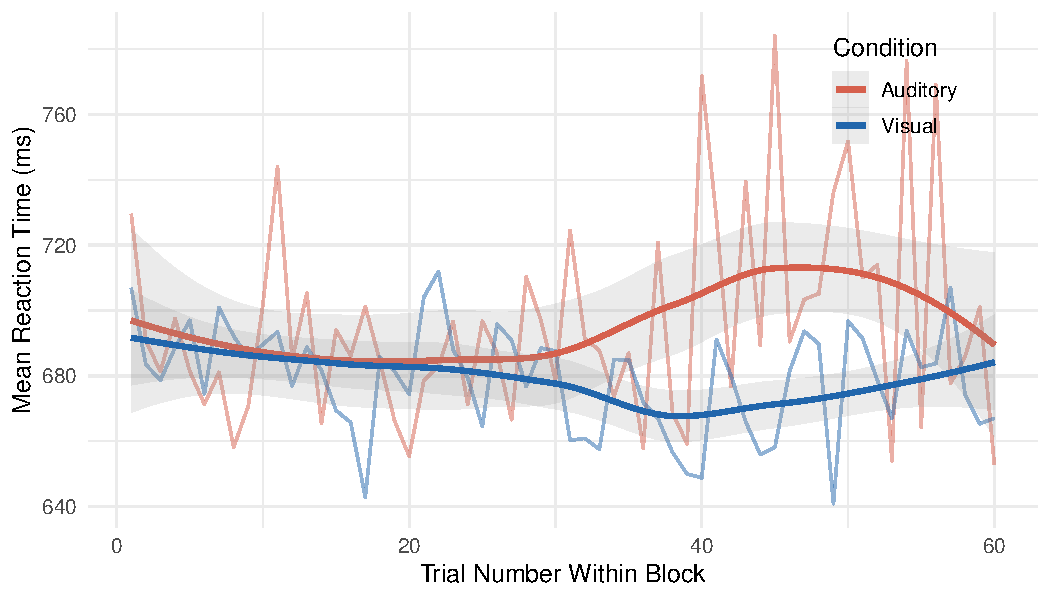
\includegraphics[width=0.75\textwidth]{learning_curve.pdf}
\caption{Mean RT by trial number within block. Both conditions show early improvement (trials 1--5) and late-block fatigue. The visual advantage is stable throughout.}
\label{fig:learning}
\end{figure}

\subsection{Tilt Effect (Error Cascading)}

When a participant missed, the probability of missing the \emph{next} trial was 24.7\% (73/295)---compared to just 3.5\% (222/6{,}324) after a hit. That is a \textbf{7$\times$ increase}, $\chi^2(1) = 293.5$, $p < .001$. Errors cascade: a single miss temporarily disrupts focus or motor calibration, triggering further misses. This ``tilt'' effect (borrowing the poker term for emotion-driven errors) operated in both conditions and is visualized in Table~\ref{tab:tilt}.

\begin{table}[H]
\centering
\caption{Tilt effect: probability of miss conditional on previous trial outcome.}
\label{tab:tilt}
\begin{tabular}{lcc}
\toprule
& \textbf{Next = Hit} & \textbf{Next = Miss} \\
\midrule
Previous = Hit & 6{,}102 (96.5\%) & 222 (3.5\%) \\
Previous = Miss & 222 (75.3\%) & 73 (24.7\%) \\
\bottomrule
\end{tabular}
\end{table}

\subsection{Spatial Click Patterns}

Figure~\ref{fig:clicks} shows all clicks plotted relative to target center. On misses, participants clicked an average of 9.1\,px below the target and 30.3\,px to the right---a systematic bias likely reflecting cursor offset or hand biomechanics.

\begin{figure}[H]
\centering
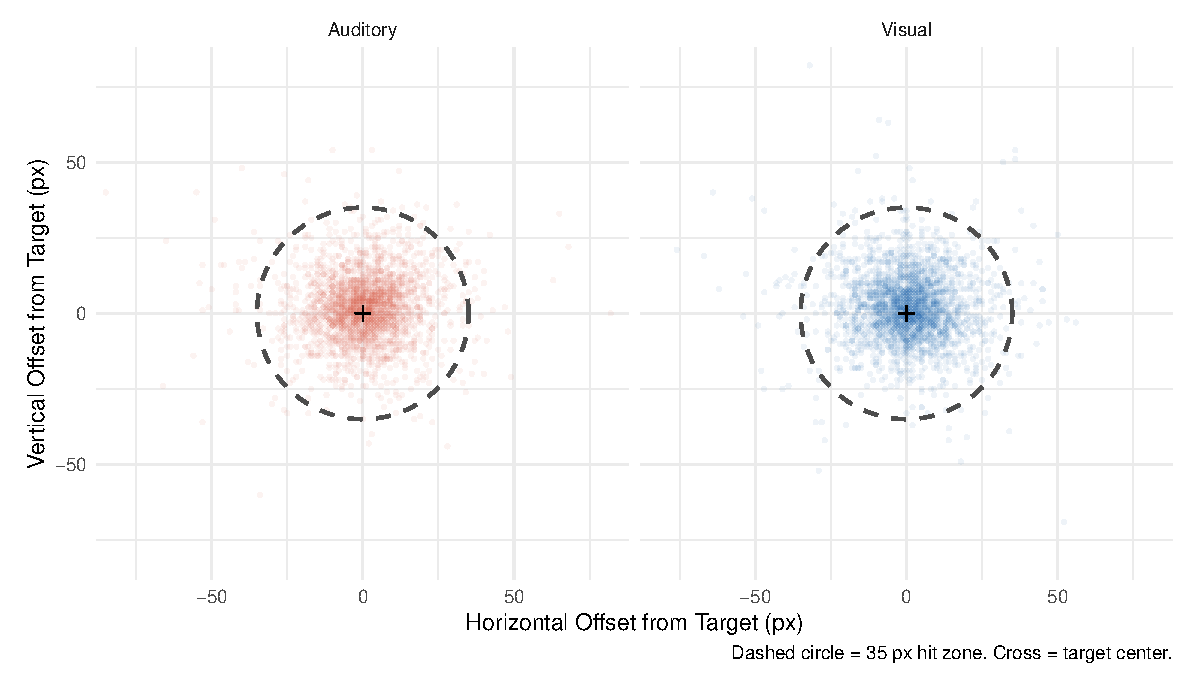
\includegraphics[width=0.85\textwidth]{click_scatter.pdf}
\caption{All clicks relative to target center, by condition. Dashed circle = 35\,px hit zone. Note the systematic offset on misses and wider scatter under visual feedback.}
\label{fig:clicks}
\end{figure}

\subsection{Counterbalancing and Block Effects}

Condition order had no significant effect on overall RT: Visual-first $M = 687$\,ms vs.\ Auditory-first $M = 689$\,ms, $t(69.7) = 0.05$, $p = .960$. Counterbalancing was effective.

Block 2 was slightly faster than Block 1 ($684$ vs.\ $692$\,ms, $p = .281$, $d = 0.13$), suggesting a small, non-significant practice effect.

\subsection{Leaderboard Engagement Effect}

A competitive leaderboard with superlative awards was introduced mid-collection. Post-leaderboard participants were 96\,ms faster ($659$ vs.\ $755$\,ms, $p < .001$) with unchanged accuracy, suggesting that gamification increased engagement without biasing the within-subject feedback comparison.


% ═══ 6. CONCLUSION ════════════════════════════════════════════
\section{Conclusion}

Neither mean RT nor mean error differed significantly between conditions (H\textsubscript{1}: $p = .151$; H\textsubscript{2}: $p = .184$). However, the \emph{structure} of the speed--accuracy tradeoff did differ (H\textsubscript{3}: $p = .023$): the SAT slope under visual feedback was 38\% steeper.

The MRT prediction---that auditory feedback should reduce interference---was not supported. Instead, the visual condition's gold/green glow created a speed incentive: participants could \emph{see} whether they were ``fast'' and were visibly frustrated at getting green instead of gold. This speed-chasing was absent in the auditory condition, where the tone distinction was less motivationally compelling. MRT's interference framework is incomplete for predicting feedback effects: modality affects not only attentional load but also \emph{motivation}.

The tilt effect ($\chi^2 = 293.5$, $p < .001$) demonstrates that trial independence cannot be assumed in sequential motor tasks: a single miss increases the next-trial miss probability by 7$\times$.

\textbf{Practical implications.} Visual feedback may inadvertently create speed pressure in safety-critical interfaces; auditory feedback may better preserve accuracy.

\textbf{Limitations.} Convenience sampling; device variability (178\,ms mouse vs.\ trackpad gap); mixed trial counts (normalized via per-participant means); uncontrolled audio environment; accuracy near ceiling ($\sim$95\%); the visual border glow is inherently more salient than a tone---our results speak to feedback ``as deployed'' rather than pure modality.

\textbf{Lessons learned.} Counterbalancing confirmed no order effect ($p = .960$). Gamification boosted engagement without biasing within-subject comparisons. The gold/green speed indicator---intended as neutral feedback---became an unintended performance incentive, which is itself evidence for the visual speed-chasing effect.


% ═══ REFERENCES ════════════════════════════════════════════════
\section*{References}
{\small
\begin{enumerate}[label={[\arabic*]},leftmargin=1.5em,itemsep=2pt]
  \item C.\,D.\ Wickens, ``Multiple resources and performance prediction,'' \emph{Theor.\ Issues Ergon.\ Sci.}, 3(2), 159--177, 2002.
  \item C.\,D.\ Wickens et al., \emph{Engineering Psychology and Human Performance}, 4th ed., Routledge, 2015.
  \item J.\ Sweller, ``Cognitive load during problem solving,'' \emph{Cognitive Science}, 12(2), 257--285, 1988.
  \item P.\,M.\ Fitts, ``Information capacity of the human motor system,'' \emph{J.\ Exp.\ Psychol.}, 47(6), 381--391, 1954.
  \item I.\,S.\ MacKenzie, ``Fitts' law as a research and design tool in HCI,'' \emph{Hum.-Comput.\ Interact.}, 7(1), 91--139, 1992.
  \item R.\,P.\ Heitz, ``The speed-accuracy tradeoff: history, physiology, methodology, and behavior,'' \emph{Front.\ Neurosci.}, 8, 150, 2014.
  \item M.\ Akamatsu et al., ``Tactile, auditory, and visual feedback in a pointing task,'' \emph{Ergonomics}, 38(4), 816--827, 1995.
  \item R.\ Sigrist et al., ``Augmented visual, auditory, haptic, and multimodal feedback in motor learning,'' \emph{Psychon.\ Bull.\ Rev.}, 20(1), 21--53, 2013.
\end{enumerate}
}


% ═══ APPENDICES ════════════════════════════════════════════════
\newpage
\appendix

\section{Assumption Checks}

\begin{itemize}
  \item RT differences: $W = 0.980$, $p = .304$ --- normal. Paired $t$-test appropriate.
  \item Error differences: $W = 0.420$, $p < .001$ --- non-normal. Wilcoxon used.
\end{itemize}

\begin{figure}[H]
\centering
\begin{subfigure}[t]{0.48\textwidth}
  \centering
  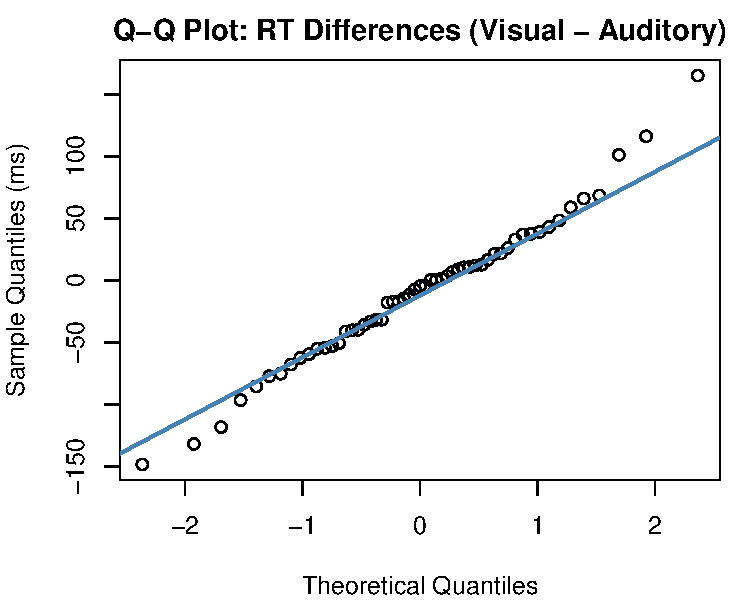
\includegraphics[width=\textwidth]{qq_rt.pdf}
  \caption{RT differences---approximately normal.}
\end{subfigure}
\hfill
\begin{subfigure}[t]{0.48\textwidth}
  \centering
  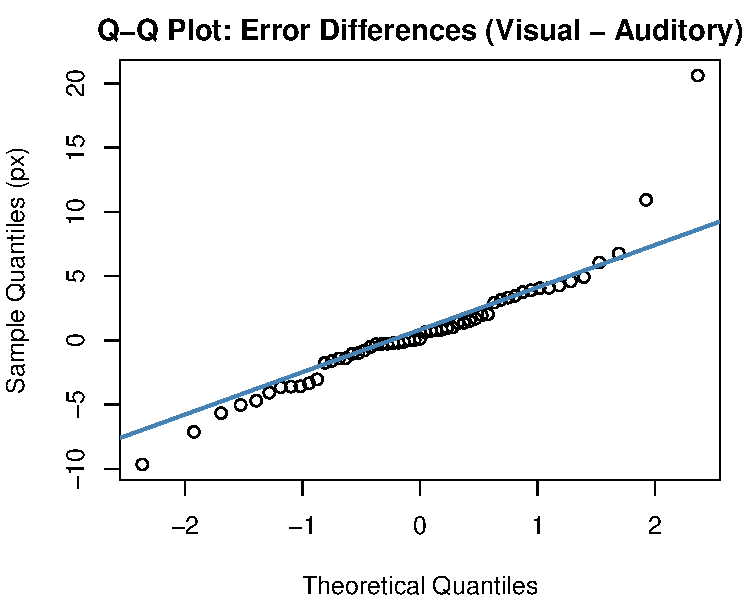
\includegraphics[width=\textwidth]{qq_error.pdf}
  \caption{Error differences---heavy tails, non-normal.}
\end{subfigure}
\caption{QQ plots for within-subject differences (visual $-$ auditory).}
\end{figure}

\begin{figure}[H]
\centering
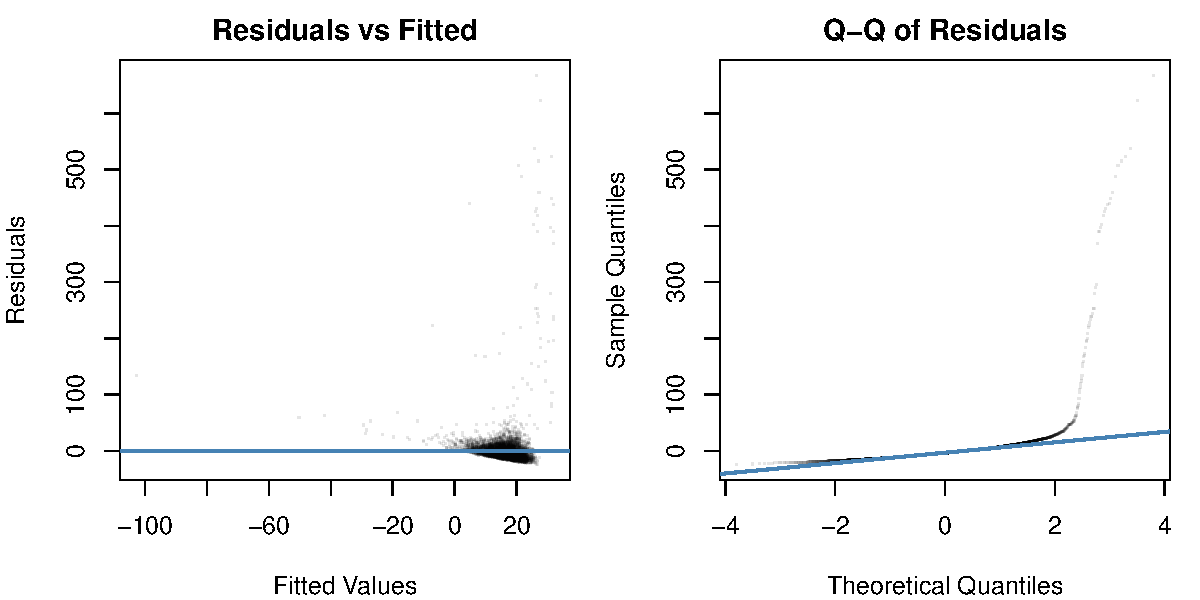
\includegraphics[width=0.85\textwidth]{residuals.pdf}
\caption{Residual diagnostics for the SAT interaction model. Funnel pattern expected with bounded error; heavy right tail from large misses.}
\end{figure}


\section{Additional Figures}

\begin{figure}[H]
\centering
\begin{subfigure}[t]{0.48\textwidth}
  \centering
  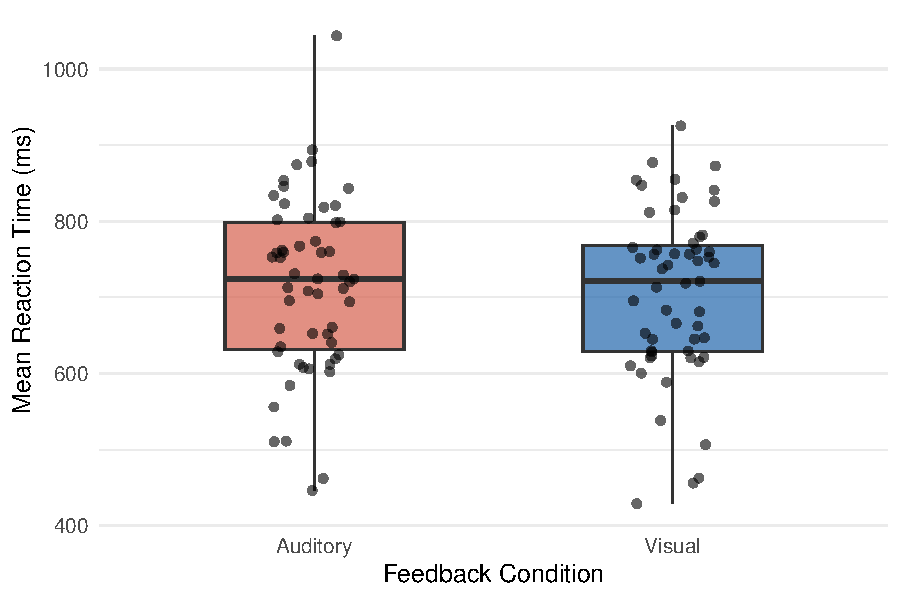
\includegraphics[width=\textwidth]{rt_boxplot.pdf}
  \caption{RT by condition with individual points.}
\end{subfigure}
\hfill
\begin{subfigure}[t]{0.48\textwidth}
  \centering
  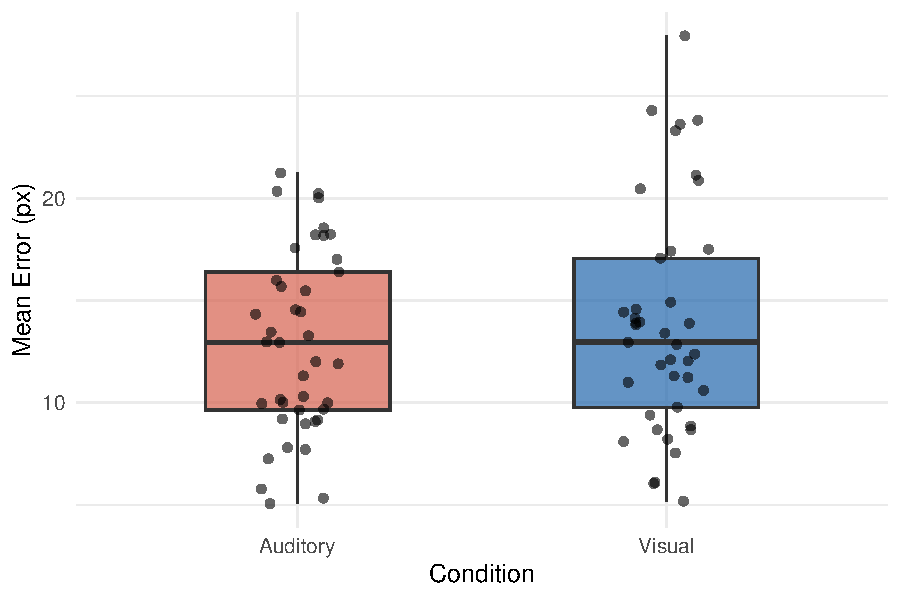
\includegraphics[width=\textwidth]{error_boxplot.pdf}
  \caption{Radial error by condition.}
\end{subfigure}
\caption{Boxplots of per-participant means by feedback condition.}
\end{figure}

\begin{figure}[H]
\centering
\begin{subfigure}[t]{0.48\textwidth}
  \centering
  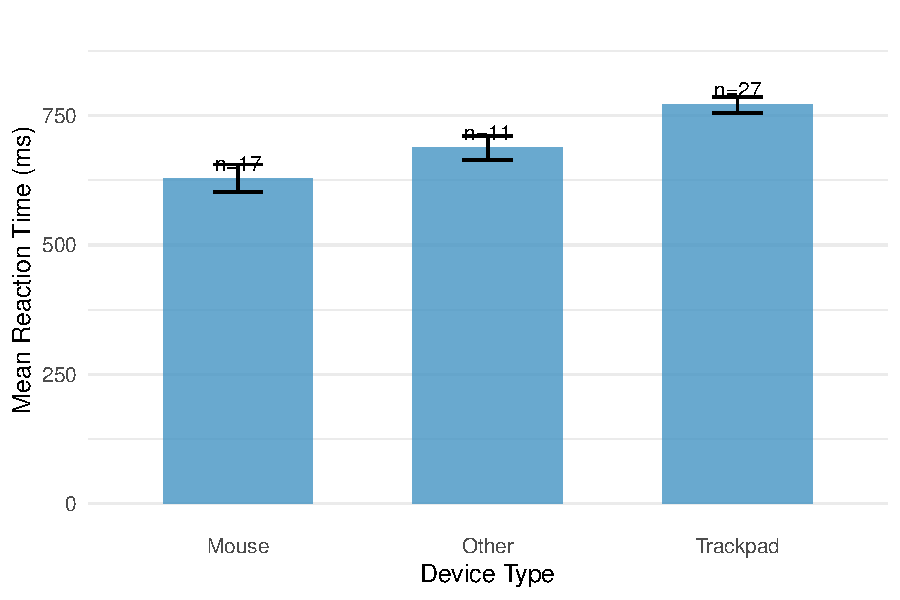
\includegraphics[width=\textwidth]{covariate_bar.pdf}
  \caption{RT by device type ($\pm$1 SE).}
\end{subfigure}
\hfill
\begin{subfigure}[t]{0.48\textwidth}
  \centering
  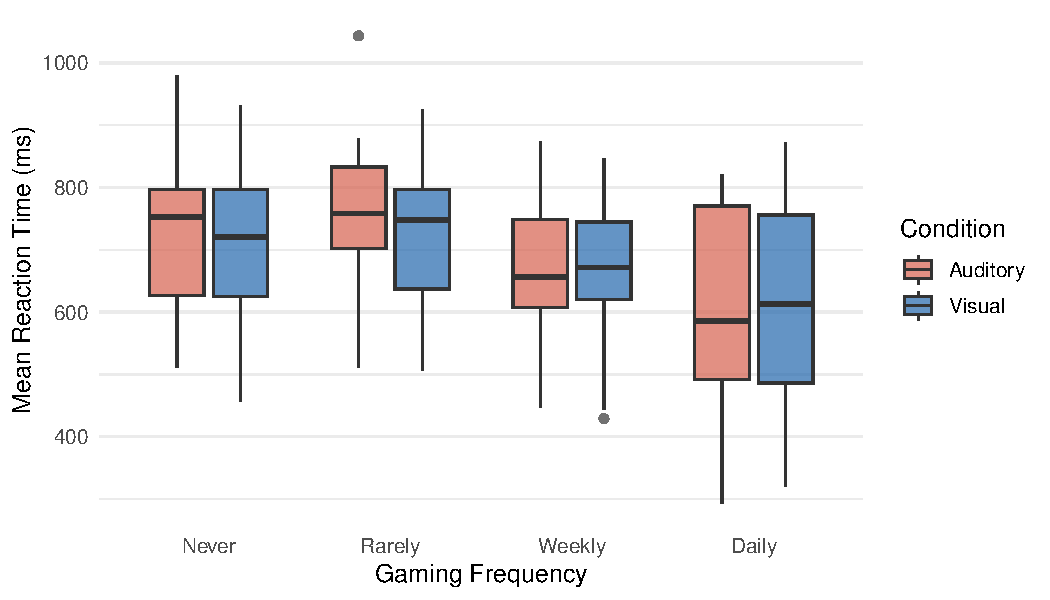
\includegraphics[width=\textwidth]{gaming_interaction.pdf}
  \caption{RT by gaming frequency and condition.}
\end{subfigure}
\caption{Covariate effects on reaction time.}
\end{figure}

\begin{figure}[H]
\centering
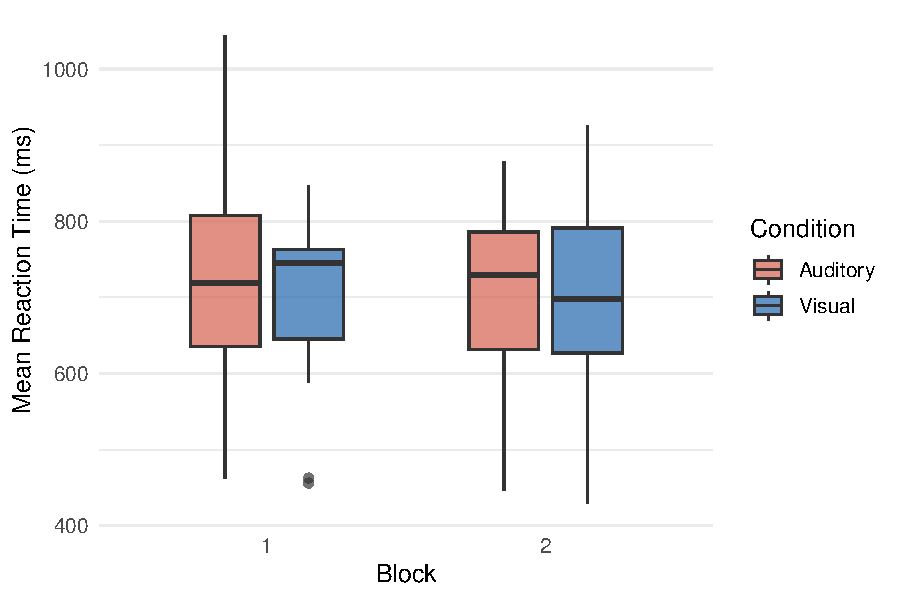
\includegraphics[width=0.7\textwidth]{block_comparison.pdf}
\caption{RT by block. Block 2 was 7.3\,ms faster ($p = .281$, $d = 0.13$).}
\end{figure}


\section{Experiment Interface}

\begin{figure}[H]
\centering
\begin{subfigure}[t]{0.48\textwidth}
  \centering
  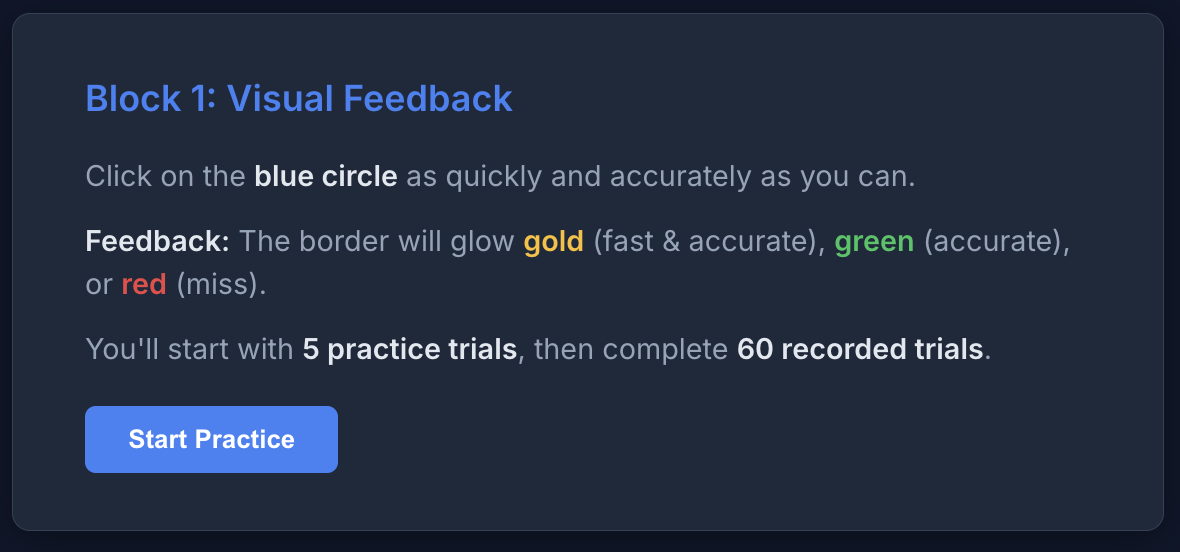
\includegraphics[width=\textwidth]{visual_information_block.png}
  \caption{Visual condition instructions.}
\end{subfigure}
\hfill
\begin{subfigure}[t]{0.48\textwidth}
  \centering
  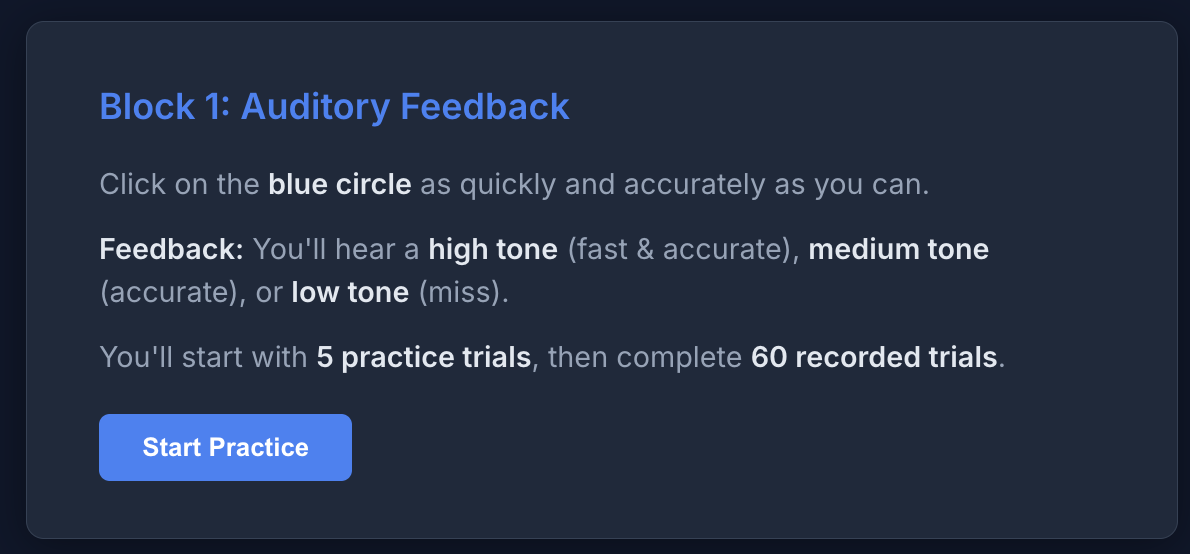
\includegraphics[width=\textwidth]{auditory_information_block.png}
  \caption{Auditory condition instructions.}
\end{subfigure}
\caption{Instruction screens. Both describe the same task; only the feedback description differs.}
\end{figure}

\begin{figure}[H]
\centering
\begin{subfigure}[t]{0.48\textwidth}
  \centering
  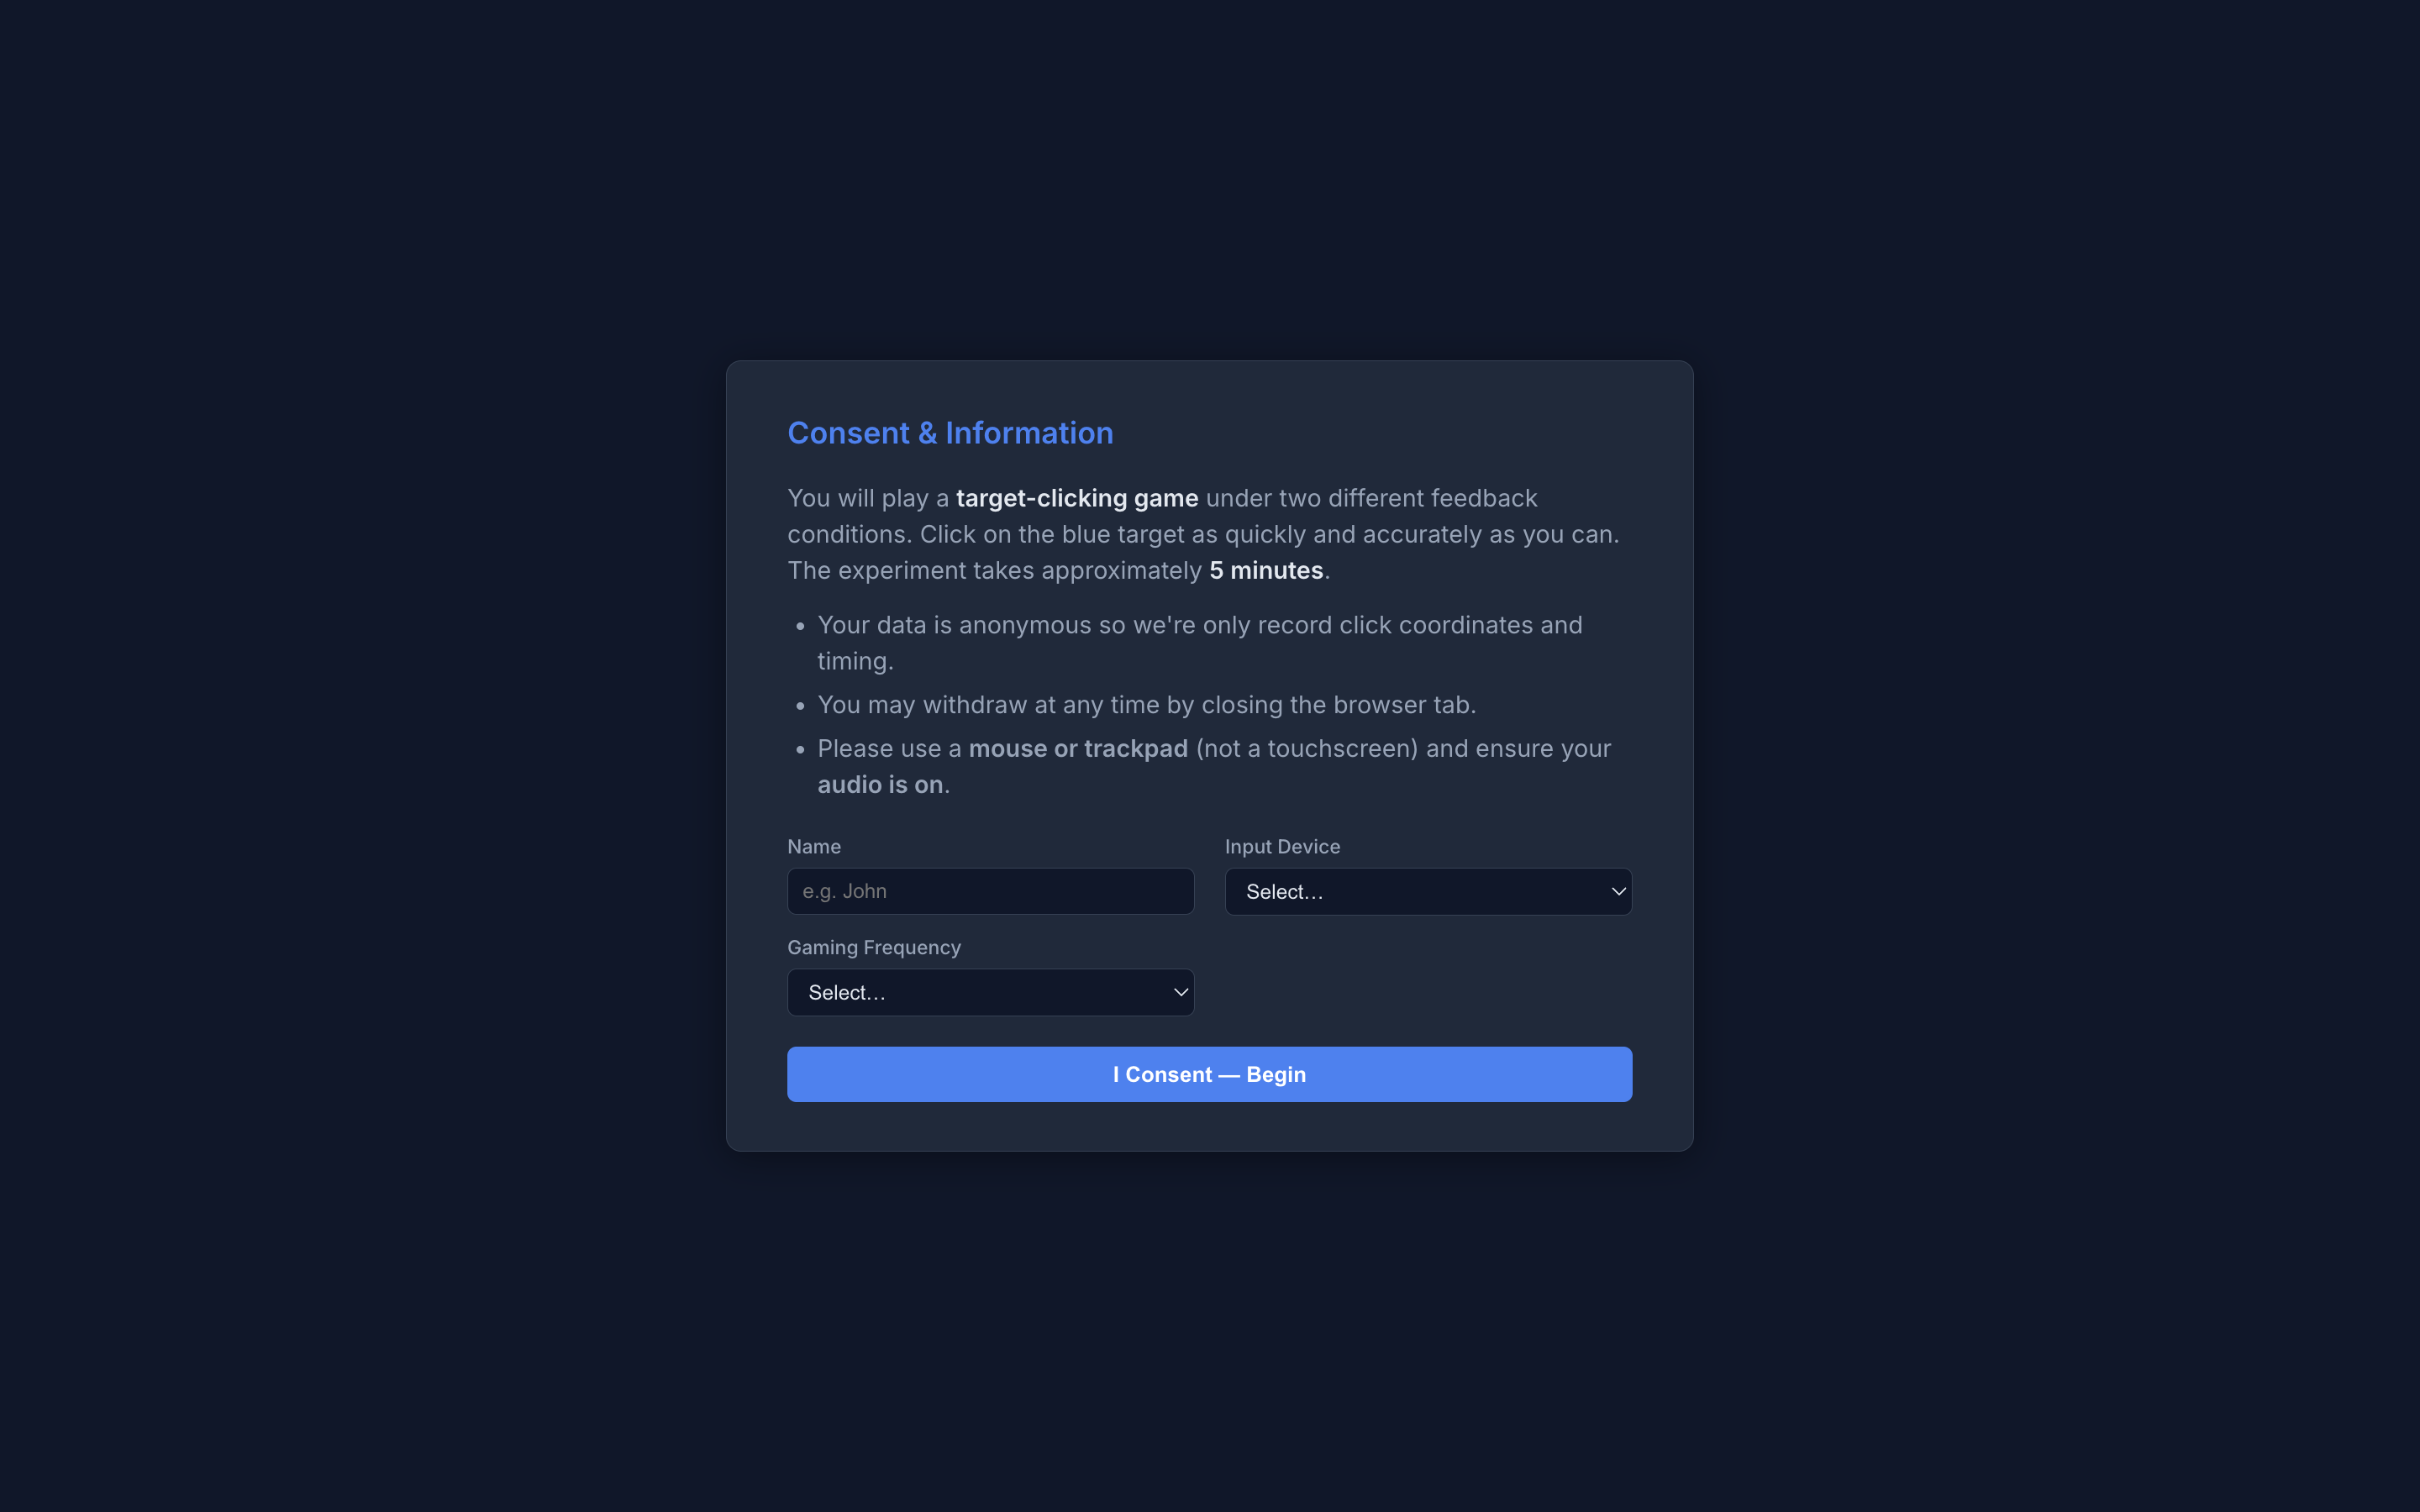
\includegraphics[width=\textwidth]{consent_screen.png}
  \caption{Consent and demographics.}
\end{subfigure}
\hfill
\begin{subfigure}[t]{0.48\textwidth}
  \centering
  
\includegraphics[width=\textwidth]{leaderboard.png}
  \caption{Leaderboard with superlatives.}
\end{subfigure}
\caption{Data collection interface. The leaderboard was introduced mid-collection to boost engagement.}
\end{figure}


\section{R Code}

All analyses were conducted in R~4.5. The pipeline consists of six scripts run sequentially via \texttt{00\_run\_all.R}:

\begin{enumerate}
  \item \texttt{01\_load\_clean.R} --- Load 72 CSVs, exclude RT outliers, aggregate per-participant means.
  \item \texttt{02\_descriptives.R} --- Summary tables by condition, device, gaming frequency.
  \item \texttt{03\_assumptions.R} --- Shapiro--Wilk tests and QQ plots.
  \item \texttt{04\_inferential.R} --- Paired $t$-test (H\textsubscript{1}), Wilcoxon (H\textsubscript{2}), multiple regression with interaction (H\textsubscript{3}).
  \item \texttt{05\_plots.R} --- All figures.
  \item \texttt{06\_secondary.R} --- Tilt effect, order check, variance, block comparison, leaderboard effect, spatial bias.
\end{enumerate}

Full code is in the \texttt{analysis/scripts/} directory submitted alongside this report.


\section{Attribution}

\begin{table}[H]
\centering
\begin{tabular}{lp{10cm}}
\toprule
\textbf{Member} & \textbf{Contributions} \\
\midrule
Markiyan Konyk & \\
Jessica Yi & \\
Memo Ozdincer & \\
\bottomrule
\end{tabular}
\end{table}

\end{document}
